\documentclass{article}
\usepackage[utf8]{inputenc}
\usepackage[margin=0.5in, driver=pdftex]{geometry}
\usepackage{xcolor}
\usepackage{amsmath}
\usepackage{graphicx}
\usepackage{relsize}
\usepackage{float}
\usepackage{svg}
\usepackage{pdflscape}
\usepackage{subfig}

\title{FIML for Channel flow (Spalart-Allmaras turbulence model)}
\author{Vishal Srivastava}
\date{}

\begin{document}

\eject \pdfpagewidth=8.5in \pdfpageheight=11.5in
%================================================================================================================================================================================
%
\maketitle
\noindent
%
Field inversion and Machine Learning framework has been used here to augment Spalart-Allmaras model to obtain correct profiles for Channel flow.
Different augmentation strategies have been proposed along with a few results. Let us first summarize the development of the Spalart-Allmaras (SA) model.
\\\\
The SA model has been calibrated using the results from fully developed mixing layers, far wake, and zero pressure gradient (ZPG) boundary layer (B/L) at
$Re=10^4$. The development goes as follows:
\begin{itemize}
    \item Take a Spalart-Allmaras working variable, $\widetilde\nu$, and consider it to be the same as eddy viscosity ($\nu_t$) for the time being. The need
          for this term will be addressed in a bit. Similarly, define a variable, $\widetilde\Omega$, and consider it to be equal to the vorticity magnitude
          ($\Omega$) for now.
    %
    \item The source term for turbulence production is modeled as the product of eddy viscosity ($\widetilde\nu$) and the vorticity magnitude ($\widetilde
          \Omega$) scaled by an appropriate coefficient ($c_{b1}$). Thus, mathematically, 
                                                    $$\mathcal{P} = c_{b1}\widetilde\nu\widetilde\Omega$$
    %
    \item It is assumed that the eddy viscosity ($\nu_t$) diffuses and is cross-produced/dissipated based on a traditional conservative diffusion term,
          $\displaystyle\frac{1}{\sigma}\nabla\cdot((\nu+\widetilde\nu)\nabla\widetilde\nu)$, and a non-conservative diffusion term, $\displaystyle\frac{c_{b2}}
          {\sigma} (\nabla\widetilde\nu)^2$. A basic mathematical analysis using the transport equation
            $$\frac{D\widetilde\nu}{Dt} = \mathcal{D},\qquad\text{where}\quad\mathcal{D} = \frac{1}{\sigma}\nabla\cdot((\nu+\widetilde\nu)\nabla\widetilde\nu) + 
                                                                                          \frac{c_{b2}}{\sigma} (\nabla\widetilde\nu)^2$$
          quickly shows that the integral of quantity $\widetilde\nu^{1+c_{b2}}$ over a large enough flow domain must remain conserved under the assumption that
          $\widetilde\nu^{1+c_{b2}}\nabla\widetilde\nu$ has a finite support (which, roughly, is always the case). There is a fair bit of analysis on the
          constraints on $c_{b2}$ and $\displaystyle\frac{1+c_{b2}}{\sigma}$ which is being skipped for now.
    %
    \item Using just these terms, possible coefficient values for $c_{b1}$, $c_{b2}$ and $\sigma$ are obtained by calibrating these against the free shear
          flow results from the fully developed mixing layer and far wake.
    %
    \item Now, we move on to the next part of the model. Firstly, let us assume that the log layer is uncompromisable for high Reynolds numbers. In this case, using 
          dimensional analysis one has the destruction term as $\displaystyle -c_{w1}\frac{\widetilde\nu^2}{d^2}$, where, to ensure log law, $\displaystyle c_{w1} = 
          \frac{c_{b1}}{\kappa^2} + \frac{1+c_{b2}}{\sigma}$.
    %
    \item This dissipation term is overly so in the outer layer resulting in an underestimation of the friction coefficient for the ZPG B/L case. A correction function
          $f_w$ is thus multiplied to the dissipation term such that it equals unity in the log layer. The definition of log layer has been set to $\displaystyle r=
          \frac{\widetilde\nu}{\widetilde\Omega\kappa^2d^2}=1$ based on which the function $f_w$ is defined as follows.
                                        $$f_w = g\left(\frac{1+c_{w3}^6}{g^6+c_{w3}^6}\right)^{1/6},\qquad\text{where}\quad g=r+c_{w2}(r^6-r)$$
          Two possible log layer preserving model augmentations in this step are mentioned as follows and have been named $c_{w2}$-augmentation and $f_w$-augmentation
              $$c_{w2}\text{-augmentation:}\qquad c_{w2}^\text{aug} = {\color{red}\beta_1^\text{FIML}\left(r,\frac{\widetilde\nu\widetilde\Omega}{\tau_w^\text{SA}}\right)} c_{w2}$$
          This comes in directly from the observation that the coefficient $c_{w2}$ was calibrated based on the ZPG B/L case at $Re=10^4$ and might be different for
          different flows and so, will be the first preference for augmentation to correct wall shear stress values. Here, $\tau_w^\text{SA}$ is the wall shear stress
          evaluated based on the solutions from the baseline SA model.
               $$f_w\text{-augmentation:}\qquad f_w^\text{aug} = {\color{red}\beta_2^\text{FIML}\left(r,\frac{\widetilde\nu\widetilde\Omega}{\tau_w^\text{SA}}\right)}(f_w-1) + 1$$
          This augmentation strategy sits a level above the previous one and can be used to correct the functional form of $f_w$ if needed. It is a rather simple and
          consistent solution as when $\beta=1$, $f_w$ remains unperturbed and in the log layer, where $f_w=1$, the new value, $f_w^\text{aug}=1$.
    %
    \item Finally, focusing on the near wall behaviour, a transformation is applied to $\widetilde\nu$ such that it is $\kappa y u_\tau$ (same as the linear relation
          for the log layer) until the log layer and $\nu_t$ outside the inner layer. A similar transformation is needed between $\widetilde\Omega$ and $\Omega$ to ensure
          the constant shear in and below the log layer. The following transformations have been defined for this purpose.
                $$\nu_t = \widetilde\nu f_{v1}, \qquad f_{v1} = \frac{\chi^3}{\chi^3+c_{v1}^3}, \qquad \chi = \frac{\widetilde\nu}{\nu}$$
                $$\widetilde\Omega = \Omega + \frac{\widetilde\nu}{\kappa^2d^2}f_{v2}, \qquad f_{v2} = 1 - \frac{\chi}{1+\chi f_{v1}}$$
          Here again, we get a chance to augment the model without meddling with any existing calibrations or the log layer. The following augmentation seems to work very well
          in correcting the buffer layer as shown in the results from channel flow configurations later in the document.
                $$\chi^\text{aug} = {\color{red}\beta_3^\text{FIML}\left(\frac{\nu}{\nu_t+\nu}\right)}\chi$$
\end{itemize}

The following types of augmentation have been attempted:
\begin{enumerate}
    \item $\displaystyle c_{w2}^\text{aug} = \beta\left(r,\quad\frac{\widetilde\nu\widetilde\Omega}{\tau_w^\text{SA}}\right) c_{w2}$
    \item $\displaystyle f_w^\text{aug} = \beta\left(r,\quad\frac{\widetilde\nu\widetilde\Omega}{\tau_w^\text{SA}}\right) f_w$
    \item $\displaystyle f_{v1}^\text{aug} = \beta\left(\frac{\nu}{\nu_t+\nu}\right) f_{v1}$
    \item $\displaystyle \mathcal{P}^\text{aug} = \beta\left(\frac{\kappa^2 d^2}{\nu}\frac{\partial u}{\partial y},\quad
                                                             \frac{\kappa^3 d^3}{\nu}\frac{\partial^2 u}{\partial y^2},\quad
                                                             \frac{\widetilde\nu\widetilde\Omega}{\tau_w^\text{SA}}\right) \mathcal{P}\qquad$ where $\mathcal{P}=\text{Production}$
\end{enumerate}
The results for the 1\textsuperscript{st} and 2\textsuperscript{nd} kind of augmentation are similar in this particular case.
%
%\begin{figure}[H]
%\centering
%\includegraphics[width=0.4\textwidth]{../figs/KOM_0550_res.png}
%\caption{Residual convergence for Re=550.0}
%\label{res}
%\end{figure}
%\eject \pdfpagewidth=8.5in \pdfpageheight=11.5in
%\end{landscape}

%---------------------------------------------------------------------------------------------------------------------------------------------------------------------------

\section*{Results}
\subsection*{FIML-Classic augmentation of the 3rd kind}
\vspace{-2em}
%==================================================================================================================
                                                                                                                  %
\begin{figure}[H]                                                                                                 %
\centering                                                                                                        %
\subfloat[][Optimization Convergence]                                                                                         %
{                                                                                                                 %
    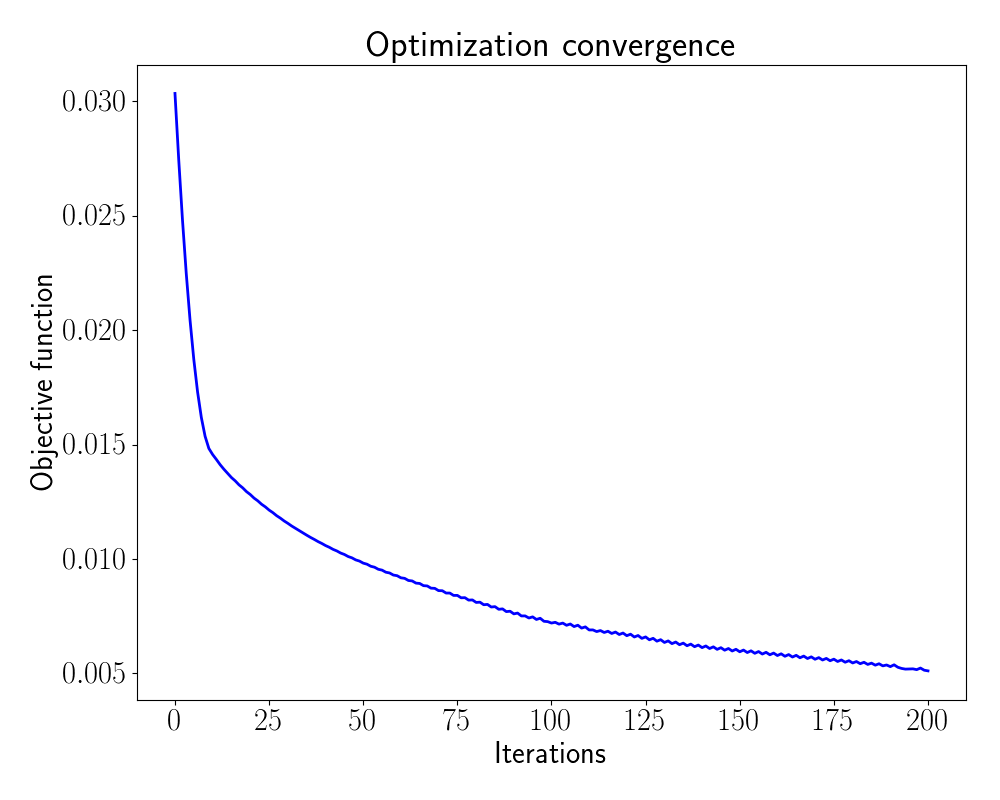
\includegraphics[width=0.32\textwidth]{images/figs/1_SA_3.png}         %
}                                                                                                                 %
%\subfloat[][ML Convergence]                                                                                        %
%{                                                                                                                 %
%    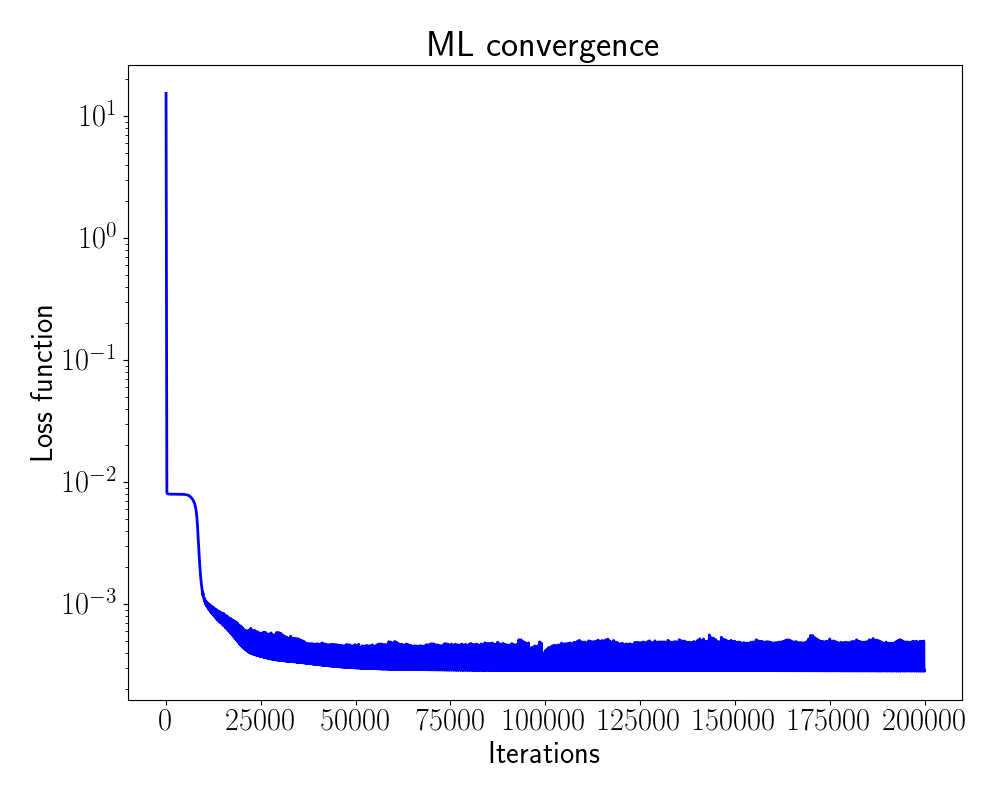
\includegraphics[width=0.32\textwidth]{images/figs/11_SA_3.png}        %
%}                                                                                                                 %
\subfloat[][Augmentation variable profile]                                                                                          %
{                                                                                                                 %
    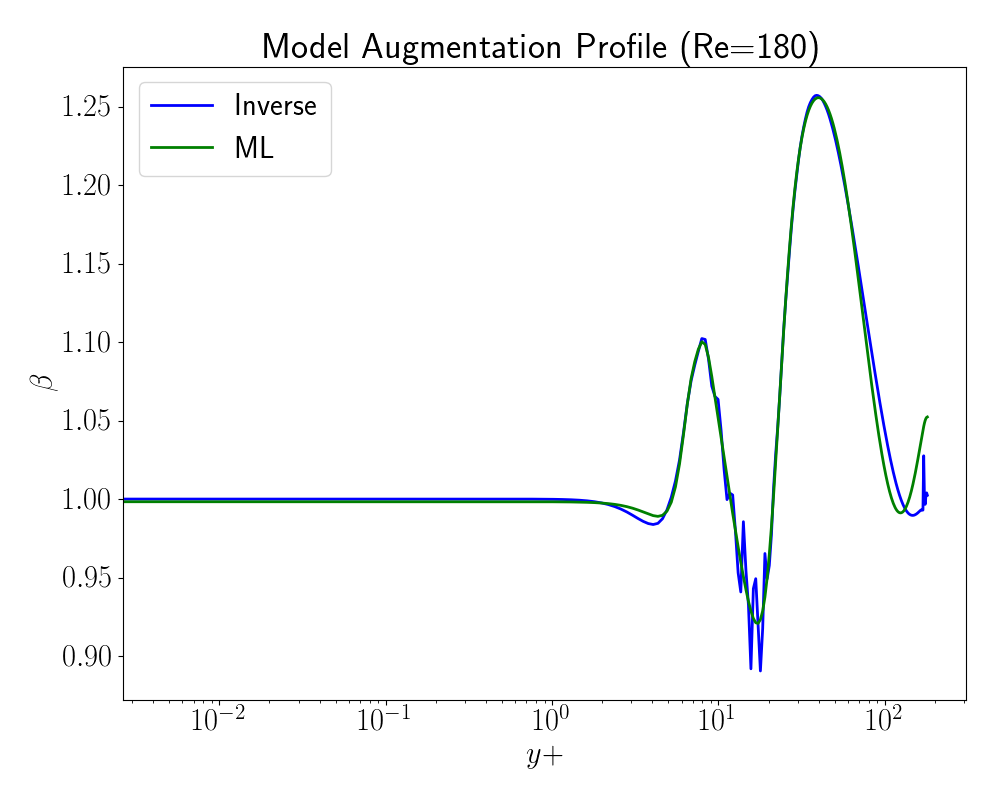
\includegraphics[width=0.32\textwidth]{images/Classic_Channel_SA_VelObj_RFtr/figs_SA_3_180/3.png}          %
}                                                                                                                 %

\subfloat[][Optimization Convergence]                                                                                         %
{                                                                                                                 %
    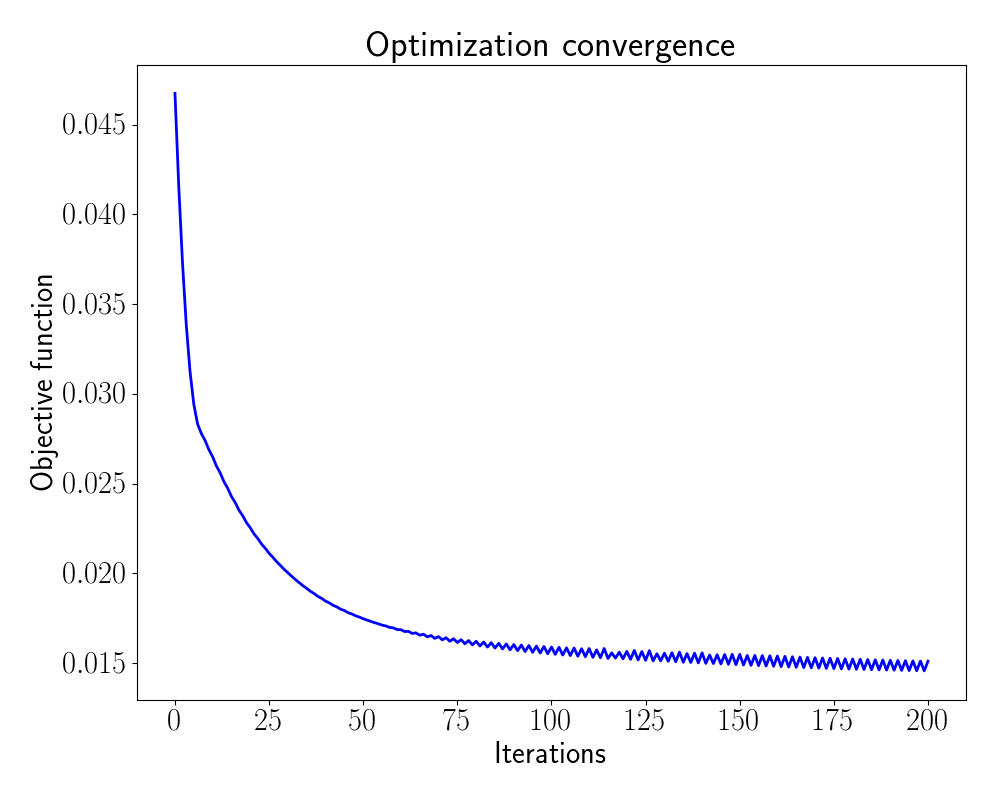
\includegraphics[width=0.32\textwidth]{images/figs/2_SA_3.png}         %
}                                                                                                                 %
%\subfloat[][ML Convergence]                                                                                        %
%{                                                                                                                 %
%    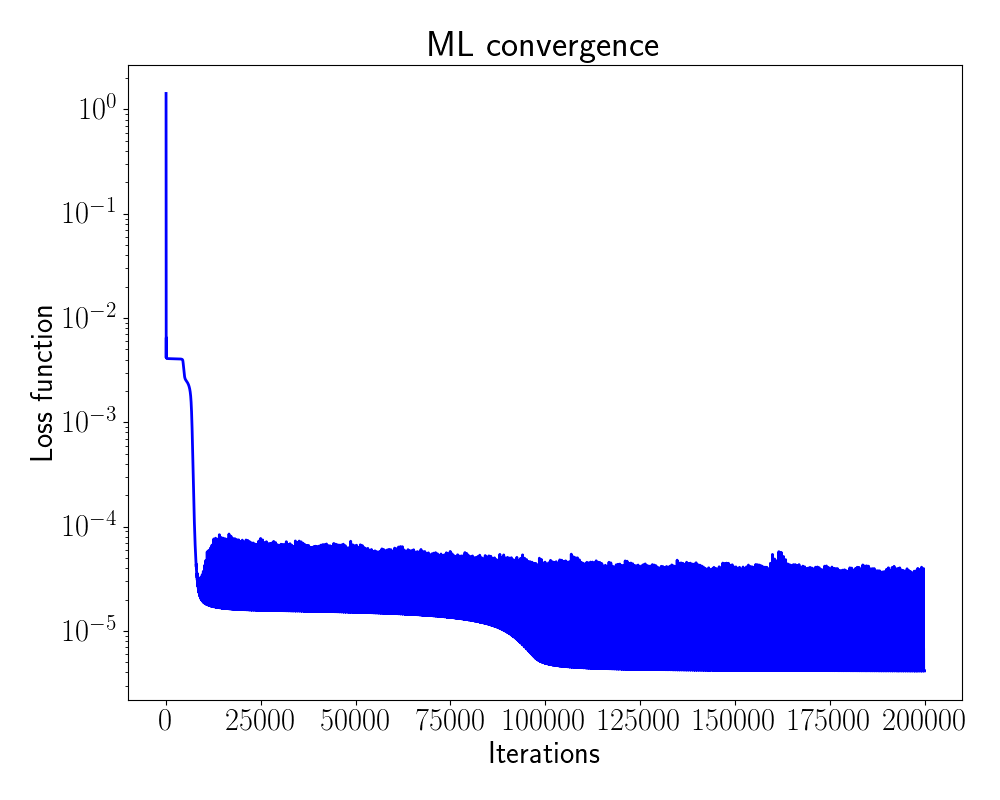
\includegraphics[width=0.32\textwidth]{images/figs/21_SA_3.png}        %
%}                                                                                                                 %
\subfloat[][Augmentation variable profile]                                                                                          %
{                                                                                                                 %
    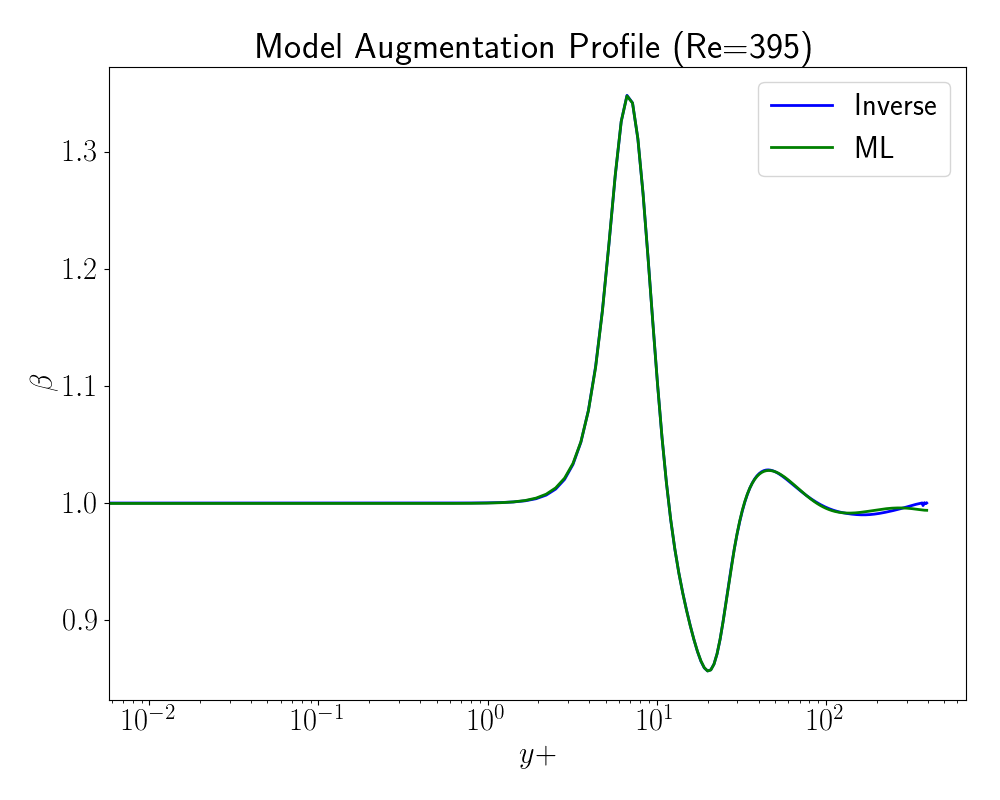
\includegraphics[width=0.32\textwidth]{images/Classic_Channel_SA_VelObj_RFtr/figs_SA_3_395/3.png}          %
}                                                                                                                 %

\subfloat[][Optimization Convergence]                                                                                         %
{                                                                                                                 %
    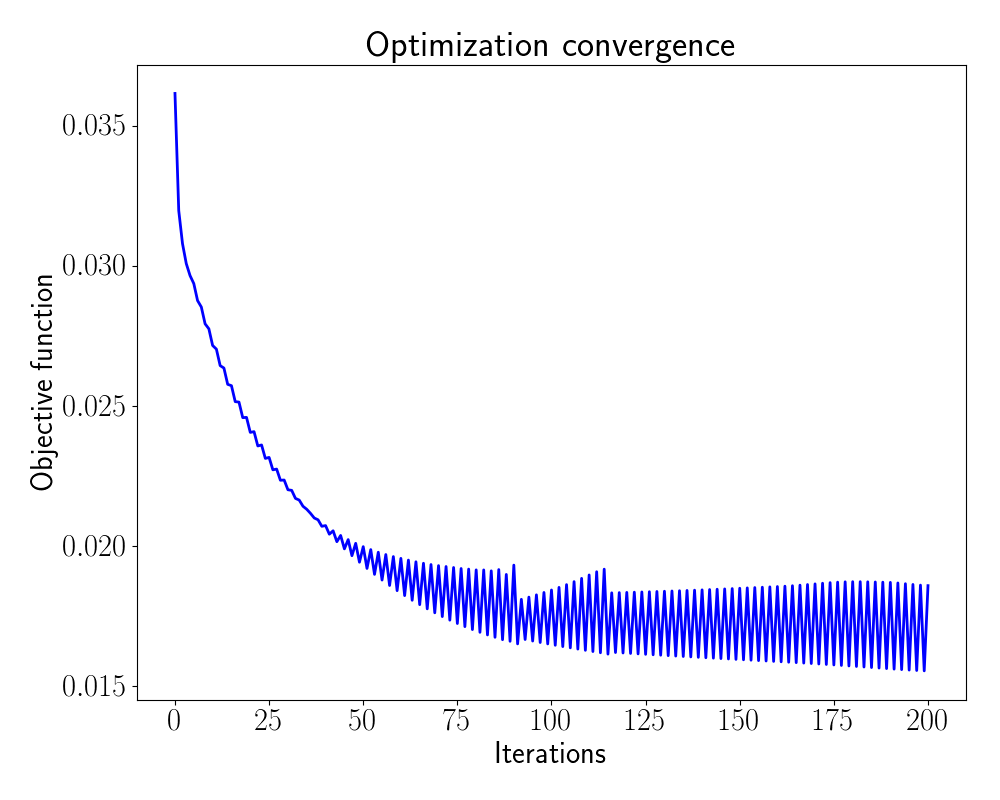
\includegraphics[width=0.32\textwidth]{images/figs/3_SA_3.png}         %
}                                                                                                                 %
%\subfloat[][ML Convergence]                                                                                        %
%{                                                                                                                 %
%    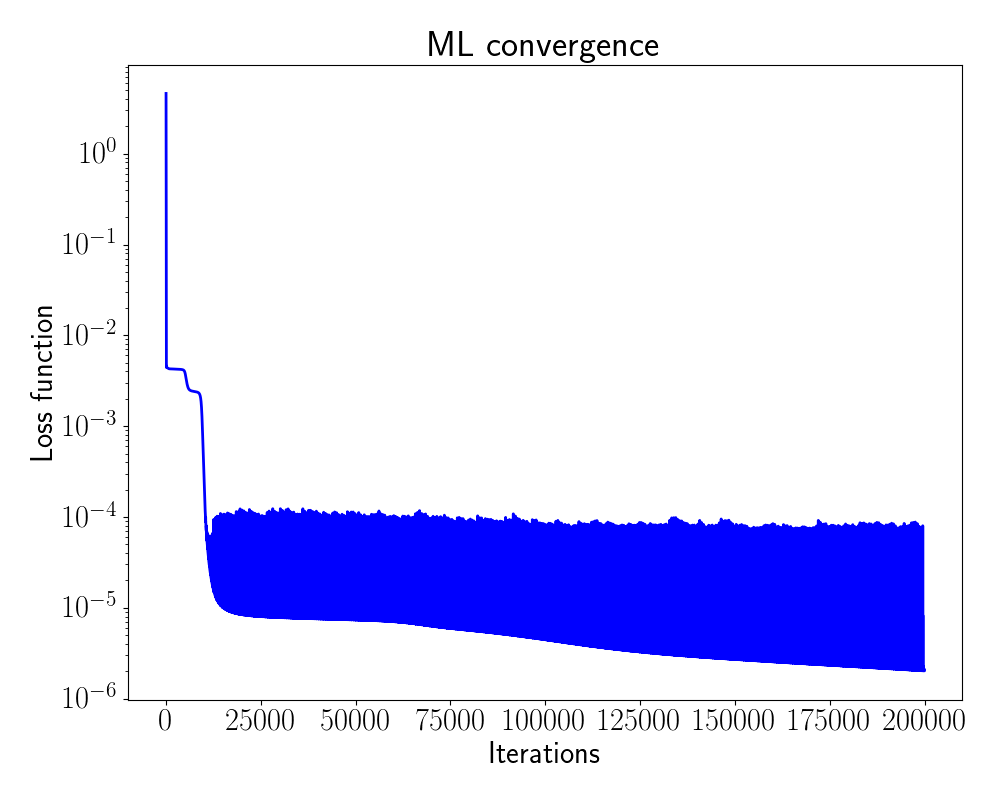
\includegraphics[width=0.32\textwidth]{images/figs/31_SA_3.png}        %
%}                                                                                                                 %
\subfloat[][Augmentation variable profile]                                                                                          %
{                                                                                                                 %
    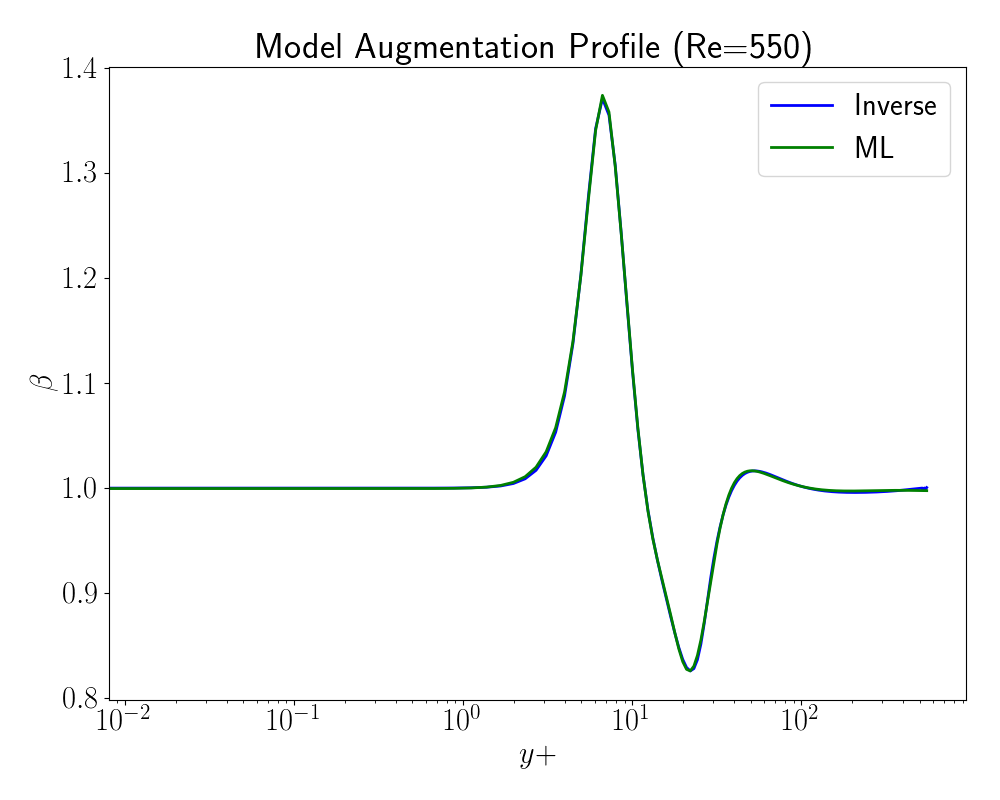
\includegraphics[width=0.32\textwidth]{images/Classic_Channel_SA_VelObj_RFtr/figs_SA_3_550/3.png}          %
}                                                                                                                 %

\subfloat[][Optimization Convergence]                                                                                         %
{                                                                                                                 %
    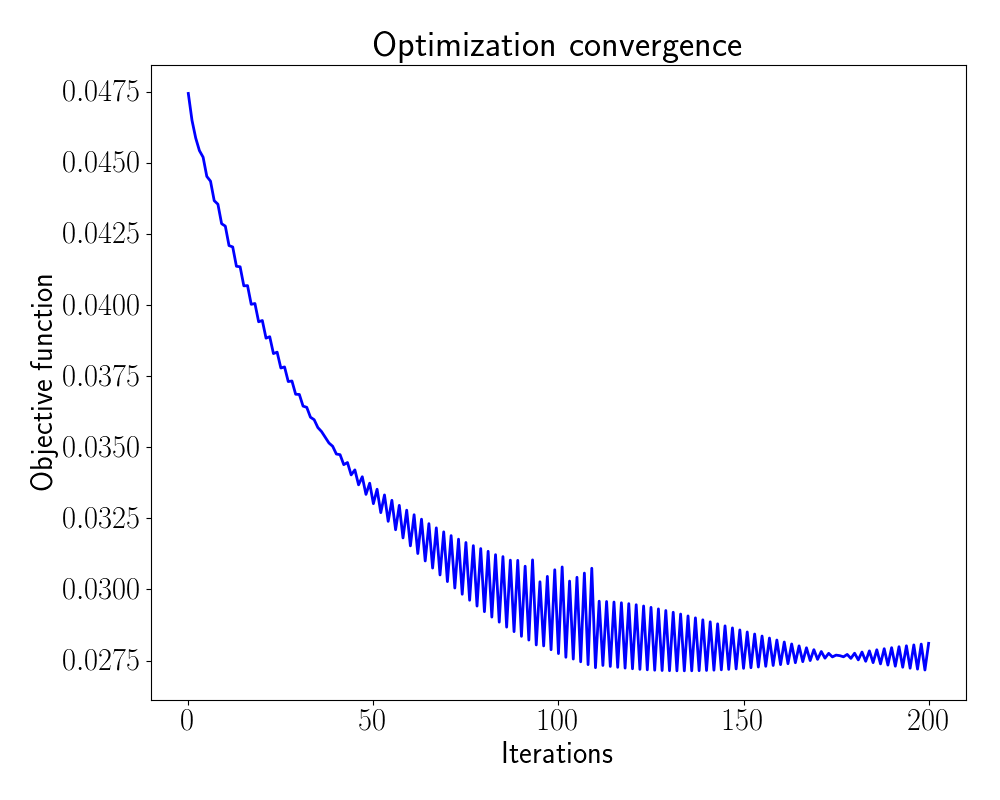
\includegraphics[width=0.32\textwidth]{images/figs/4_SA_3.png}         %
}                                                                                                                 %
%\subfloat[][ML Convergence]                                                                                        %
%{                                                                                                                 %
%    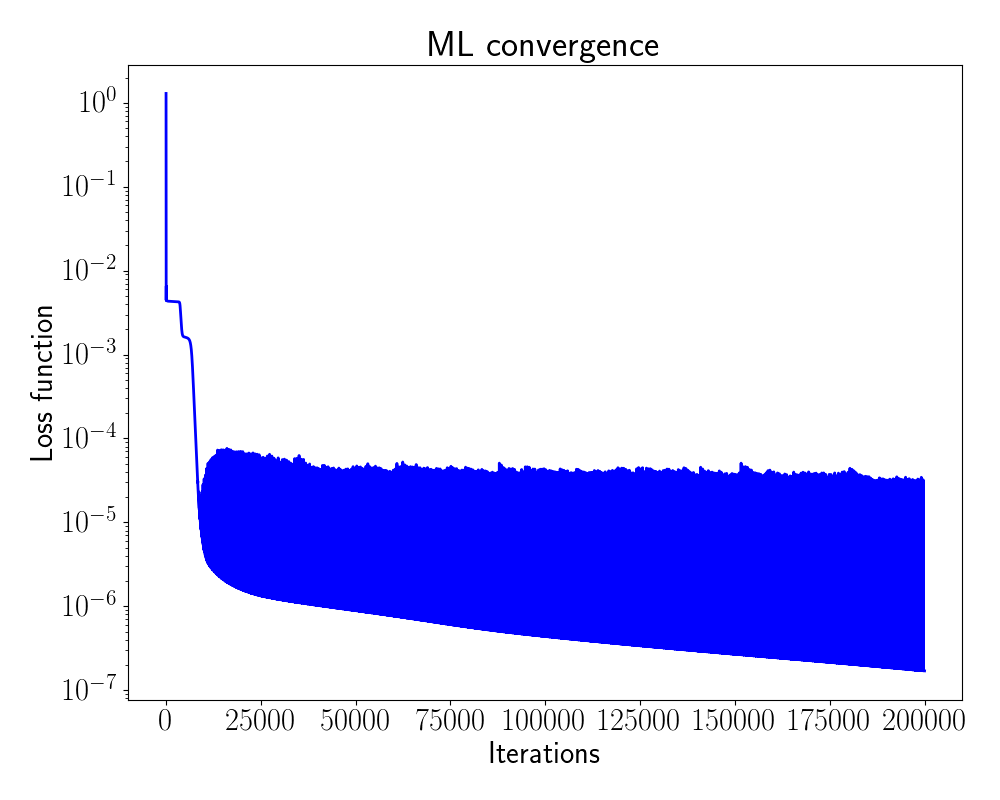
\includegraphics[width=0.32\textwidth]{images/figs/41_SA_3.png}        %
%}                                                                                                                 %
\subfloat[][Augmentation variable profile]                                                                                          %
{                                                                                                                 %
    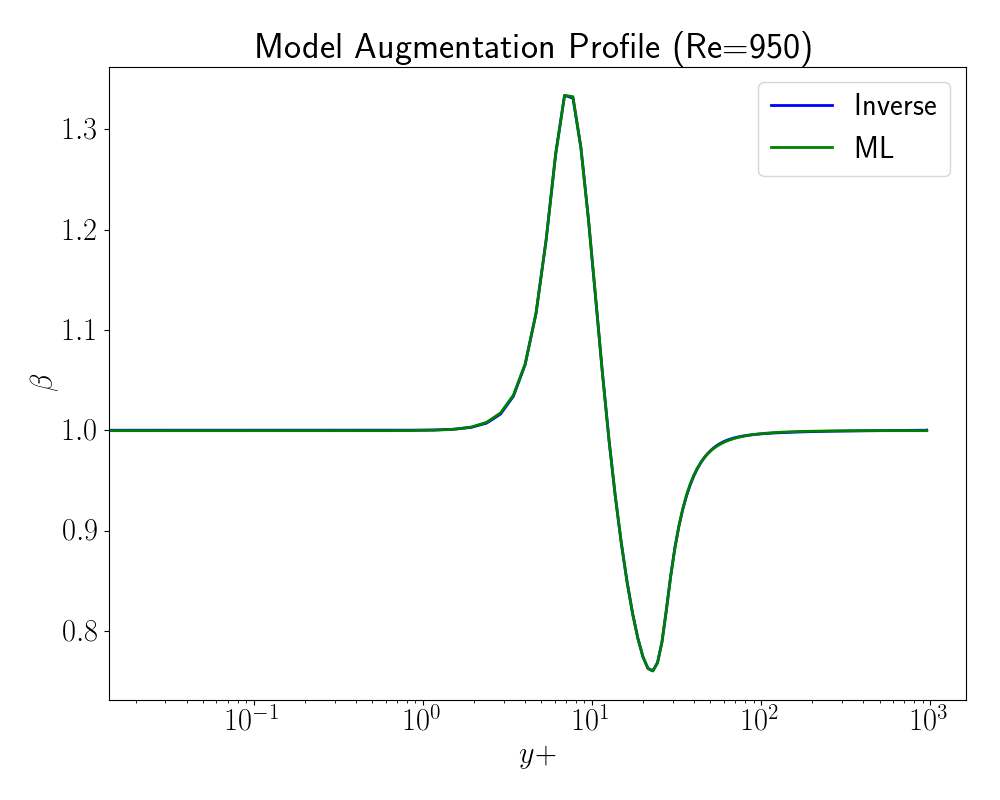
\includegraphics[width=0.32\textwidth]{images/Classic_Channel_SA_VelObj_RFtr/figs_SA_3_950/3.png}          %
}                                                                                                                 %
                                                                                                                  %
\caption{Convergence and beta plots}                                                                                       %
\label{convbeta2}                                                                                                     %
\end{figure}                                                                                                      %
                                                                                                                  %
%==================================================================================================================
%==================================================================================================================
                                                                                                                  %
\begin{figure}[H]                                                                                                 %
\centering                                                                                                        %
\subfloat[][Optimization Convergence]                                                                                         %
{                                                                                                                 %
    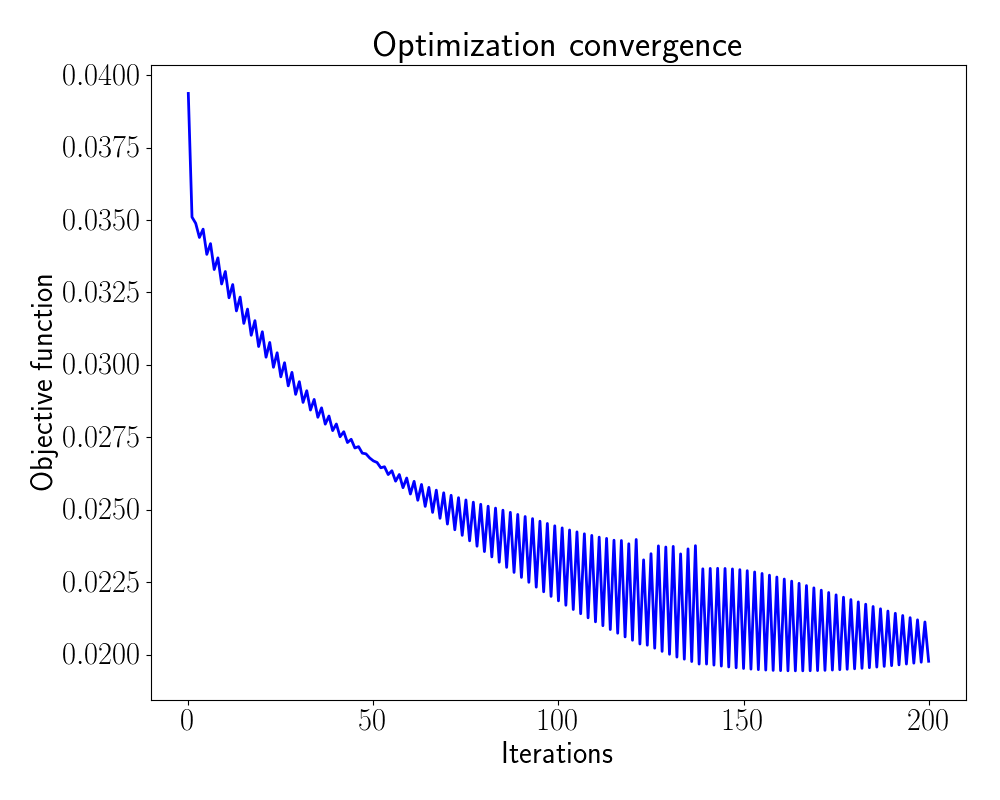
\includegraphics[width=0.32\textwidth]{images/figs/5_SA_3.png}         %
}                                                                                                                 %
%\subfloat[][ML Convergence]                                                                                        %
%{                                                                                                                 %
%    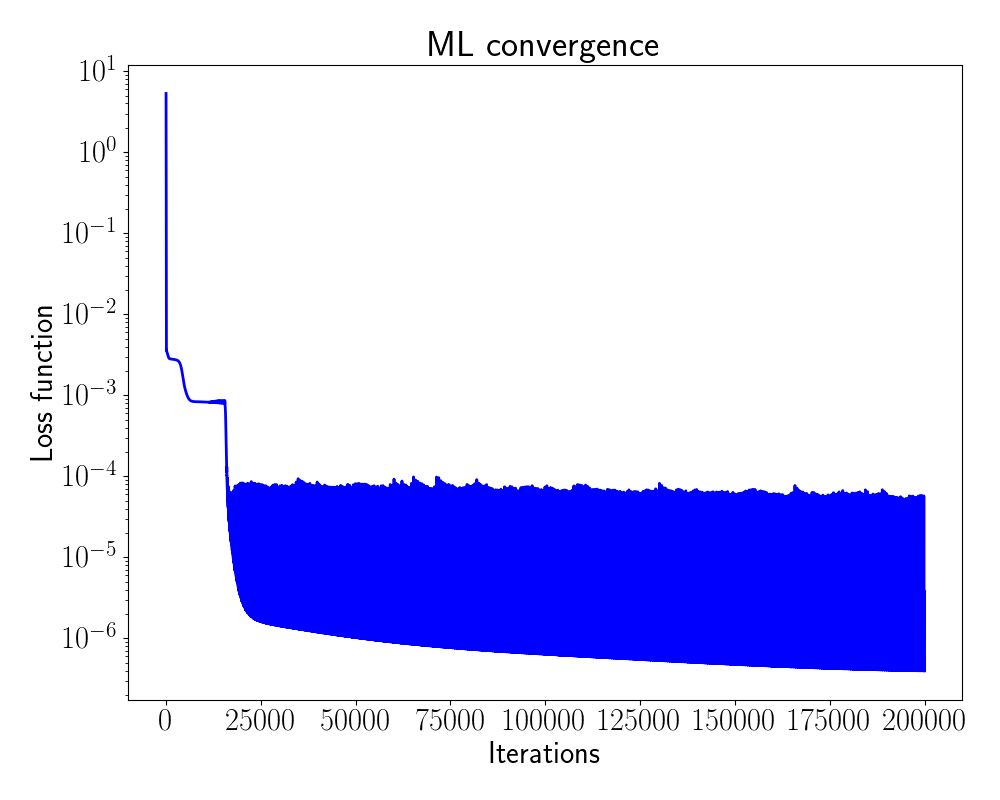
\includegraphics[width=0.32\textwidth]{images/figs/51_SA_3.png}        %
%}                                                                                                                 %
\subfloat[][Augmentation variable profile]                                                                                          %
{                                                                                                                 %
    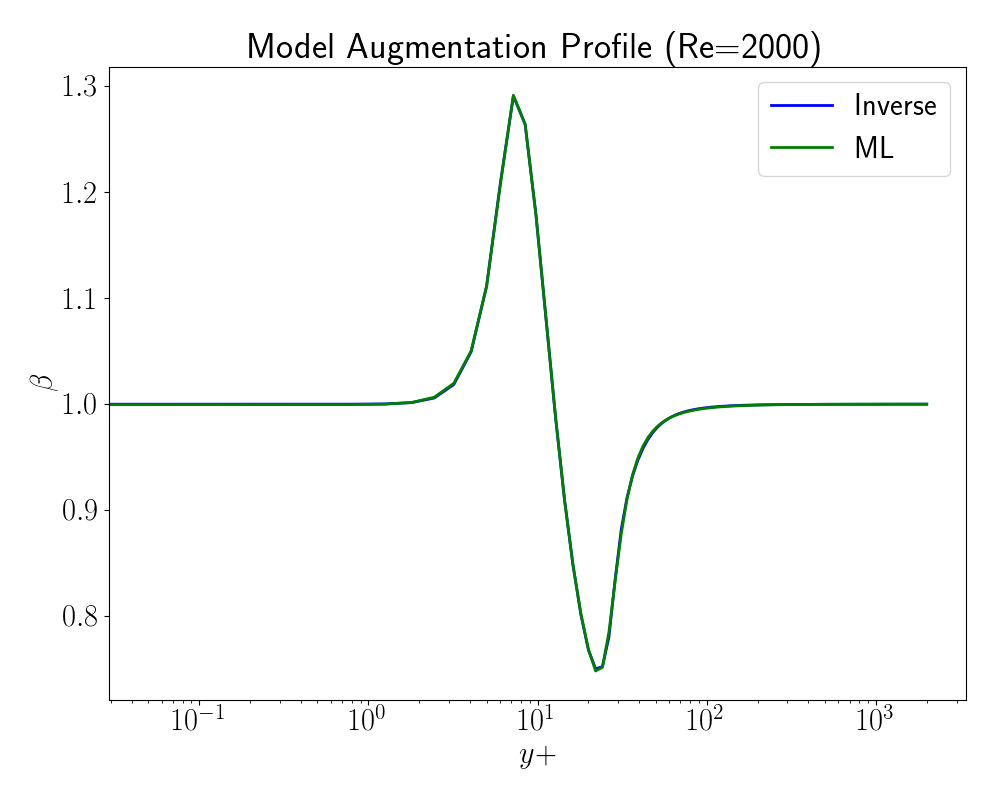
\includegraphics[width=0.32\textwidth]{images/Classic_Channel_SA_VelObj_RFtr/figs_SA_3_2000/3.png}          %
}                                                                                                                 %

\subfloat[][Optimization Convergence]                                                                                         %
{                                                                                                                 %
    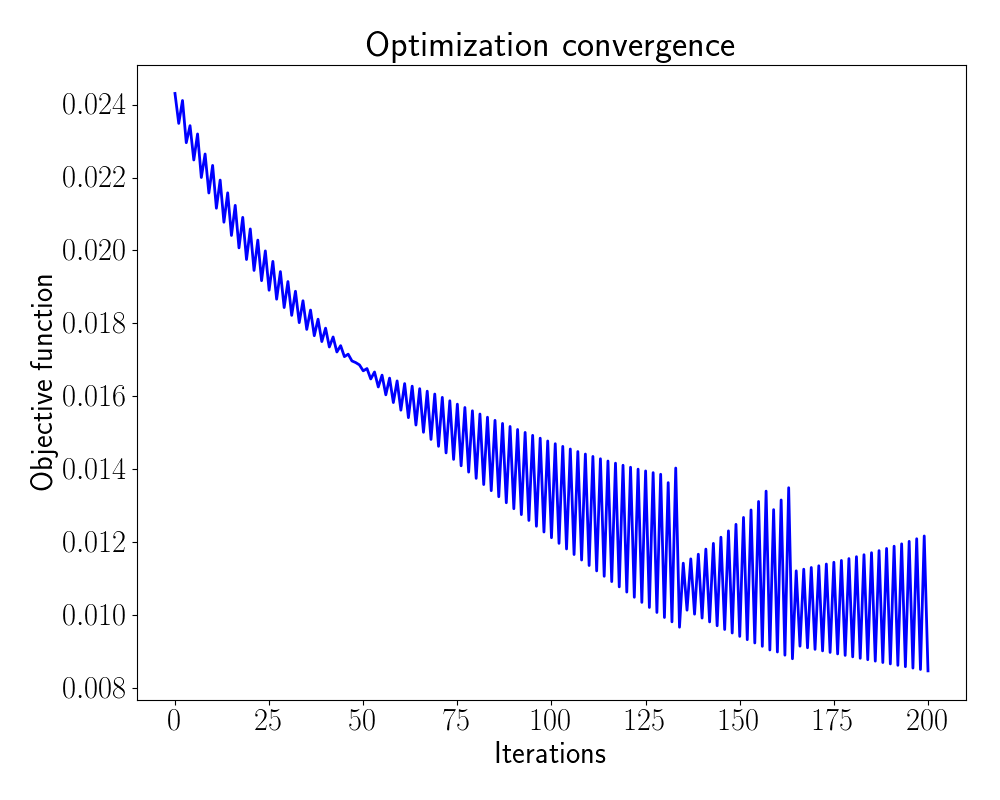
\includegraphics[width=0.32\textwidth]{images/figs/6_SA_3.png}         %
}                                                                                                                 %
%\subfloat[][ML Convergence]                                                                                        %
%{                                                                                                                 %
%    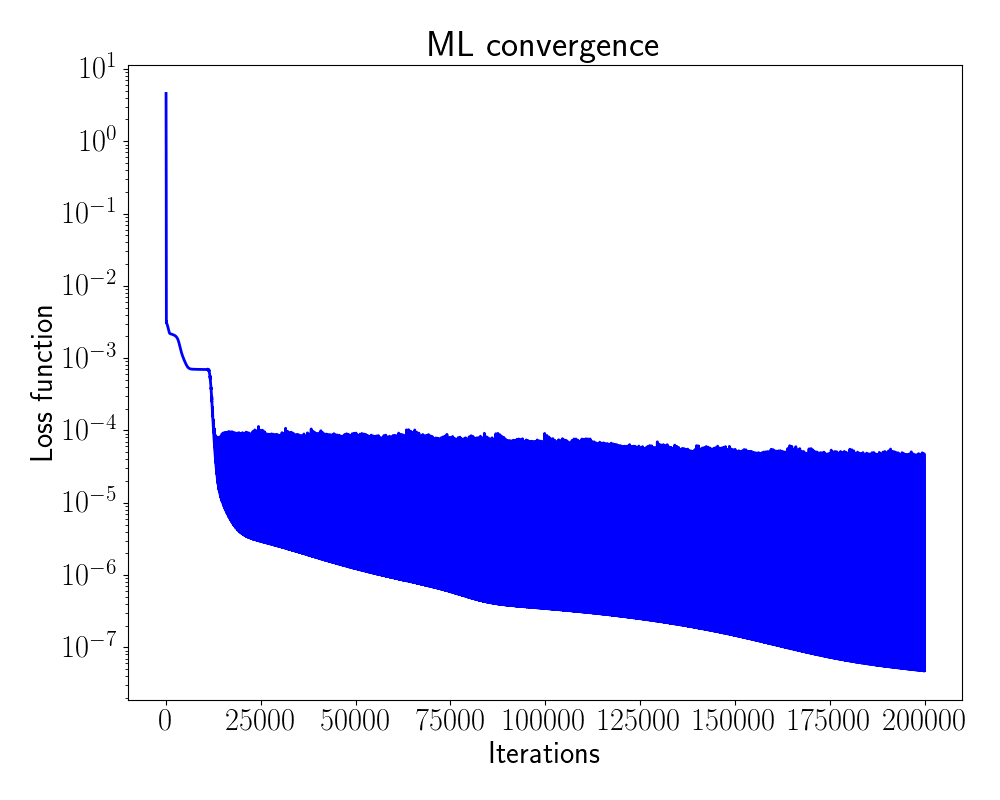
\includegraphics[width=0.32\textwidth]{images/figs/61_SA_3.png}        %
%}                                                                                                                 %
\subfloat[][Augmentation variable profile]                                                                                          %
{                                                                                                                 %
    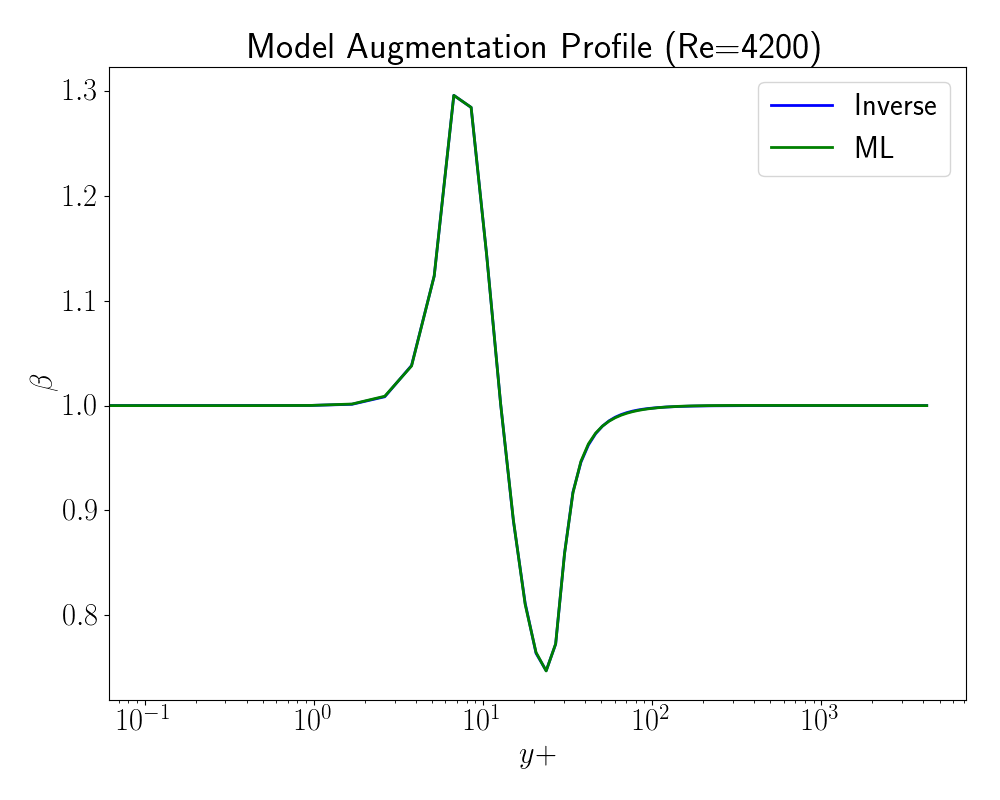
\includegraphics[width=0.32\textwidth]{images/Classic_Channel_SA_VelObj_RFtr/figs_SA_3_4200/3.png}          %
}                                                                                                                 %

\subfloat[][Optimization Convergence]                                                                                         %
{                                                                                                                 %
    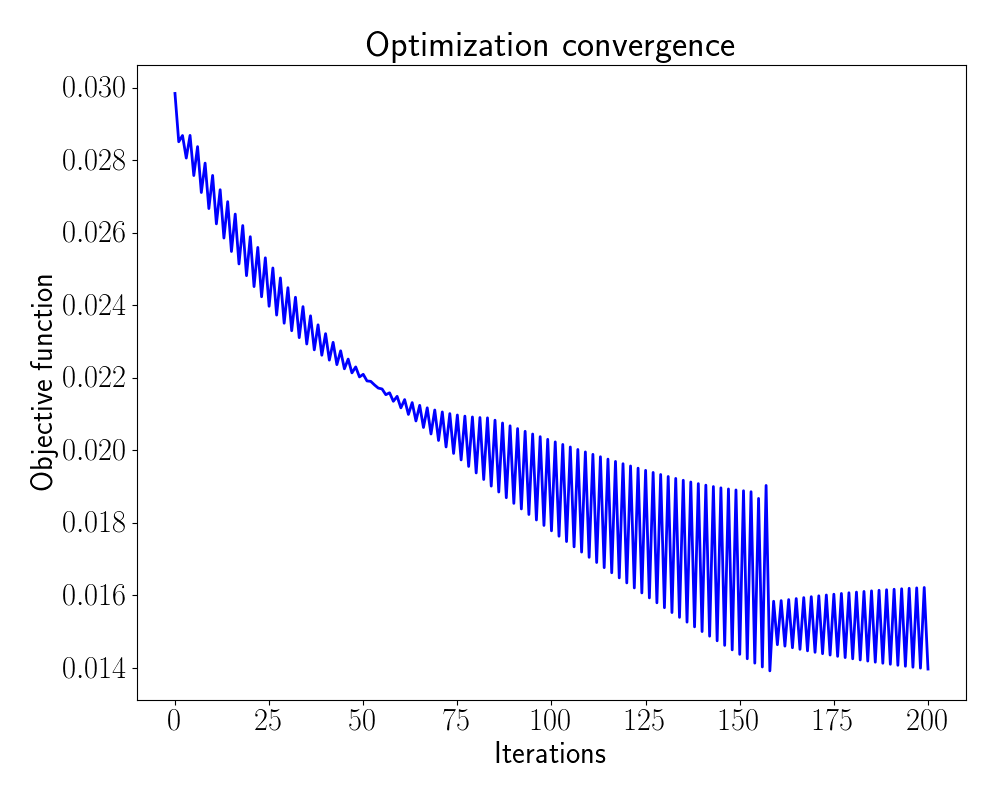
\includegraphics[width=0.32\textwidth]{images/figs/7_SA_3.png}         %
}                                                                                                                 %
%\subfloat[][ML Convergence]                                                                                        %
%{                                                                                                                 %
%    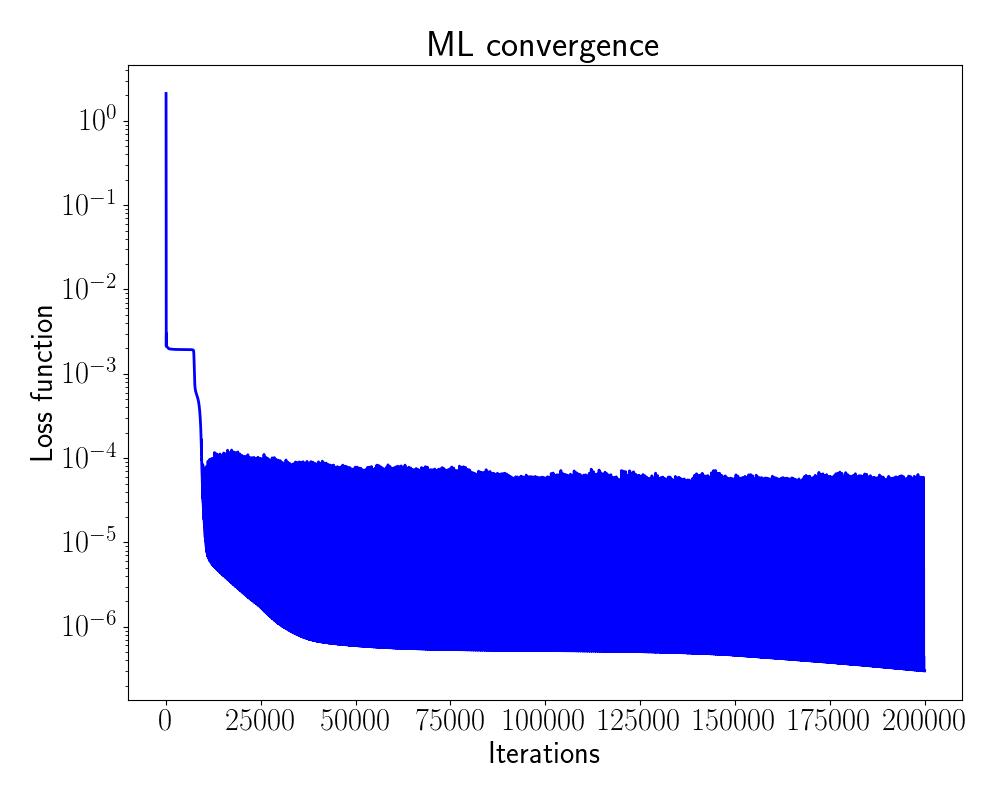
\includegraphics[width=0.32\textwidth]{images/figs/71_SA_3.png}        %
%}                                                                                                                 %
\subfloat[][Augmentation variable profile]                                                                                          %
{                                                                                                                 %
    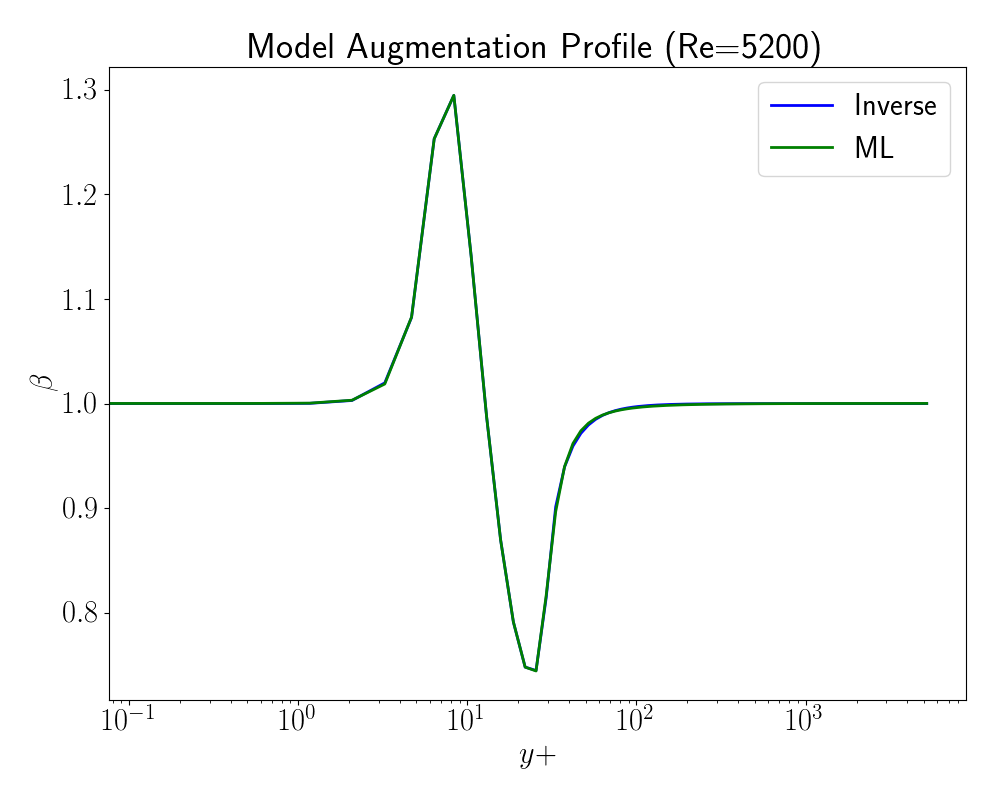
\includegraphics[width=0.32\textwidth]{images/Classic_Channel_SA_VelObj_RFtr/figs_SA_3_5200/3.png}          %
}                                                                                                                 %

\caption{Convergence and beta plots}                                                                                       %
\label{convbeta1}                                                                                                     %
\end{figure}                                                                                                      %
                                                                                                                  %
%==================================================================================================================
\pagebreak
%==================================================================================================================
                                                                                                                  %
\begin{figure}[H]                                                                                                 %
\centering                                                                                                        %
\subfloat[][Velocity profile]                                                                                          %
{                                                                                                                 %
    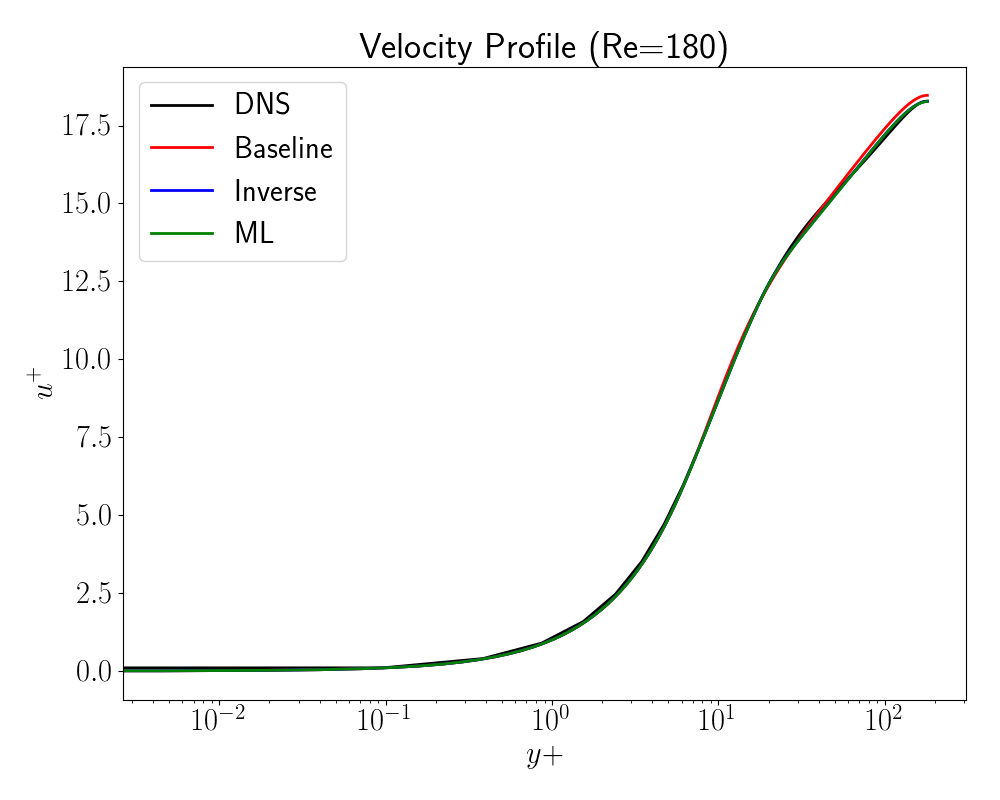
\includegraphics[width=0.32\textwidth]{images/Classic_Channel_SA_VelObj_RFtr/figs_SA_3_180/1.png}          %
}                                                                                                                 %
\subfloat[][Velocity Gradient profile]                                                                                          %
{                                                                                                                 %
    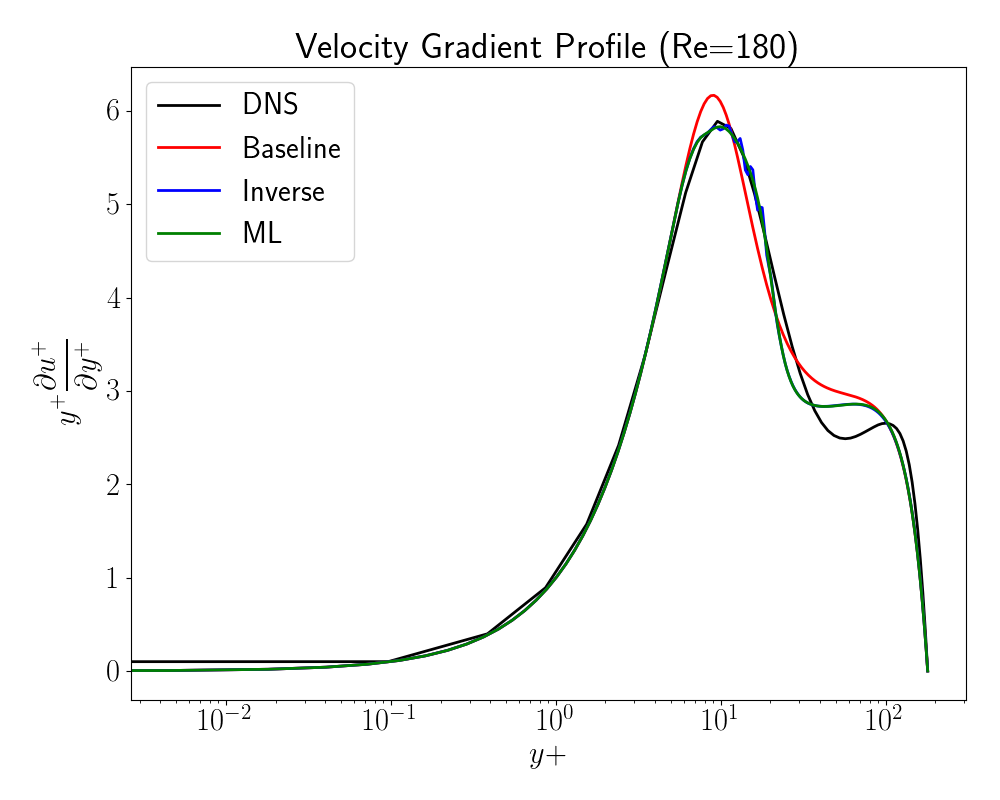
\includegraphics[width=0.32\textwidth]{images/Classic_Channel_SA_VelObj_RFtr/figs_SA_3_180/2.png}          %
}                                                                                                                 %

\subfloat[][Velocity profile]                                                                                          %
{                                                                                                                 %
    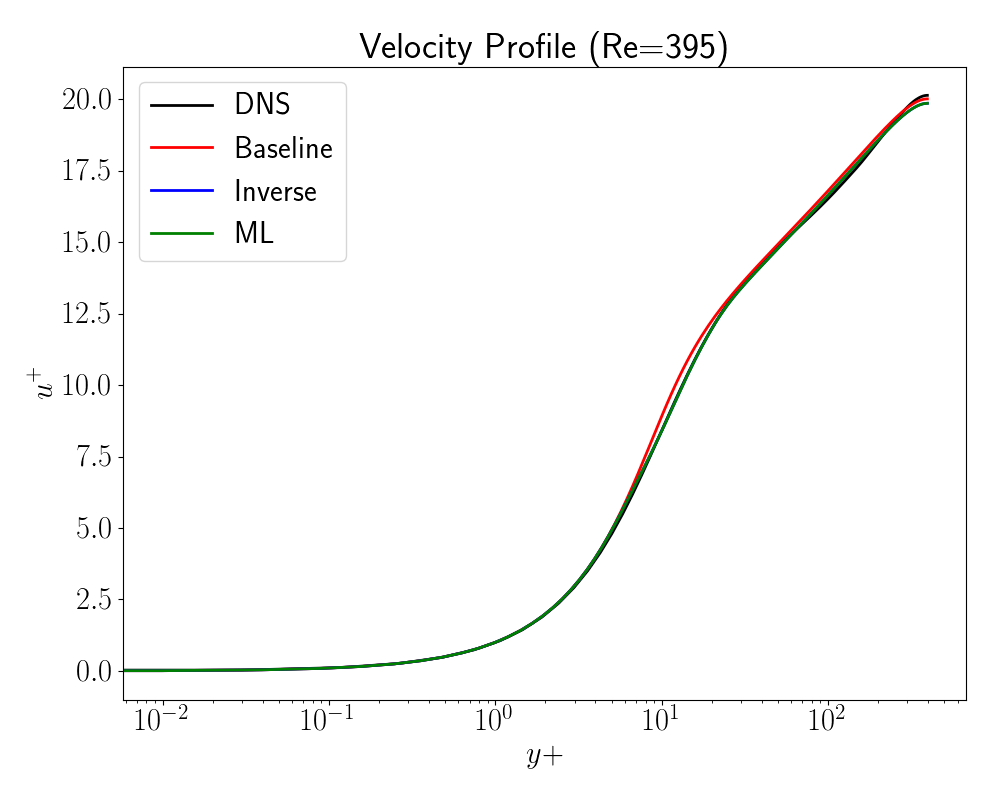
\includegraphics[width=0.32\textwidth]{images/Classic_Channel_SA_VelObj_RFtr/figs_SA_3_395/1.png}          %
}                                                                                                                 %
\subfloat[][Velocity Gradient profile]                                                                                          %
{                                                                                                                 %
    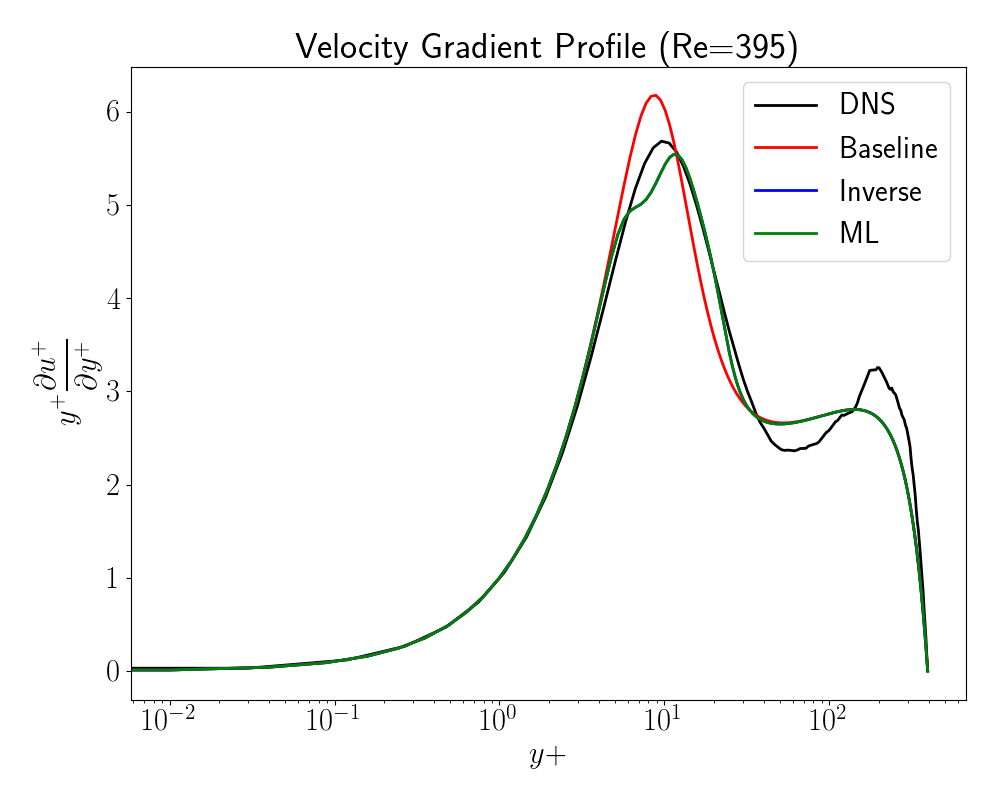
\includegraphics[width=0.32\textwidth]{images/Classic_Channel_SA_VelObj_RFtr/figs_SA_3_395/2.png}          %
}                                                                                                                 %

\subfloat[][Velocity profile]                                                                                          %
{                                                                                                                 %
    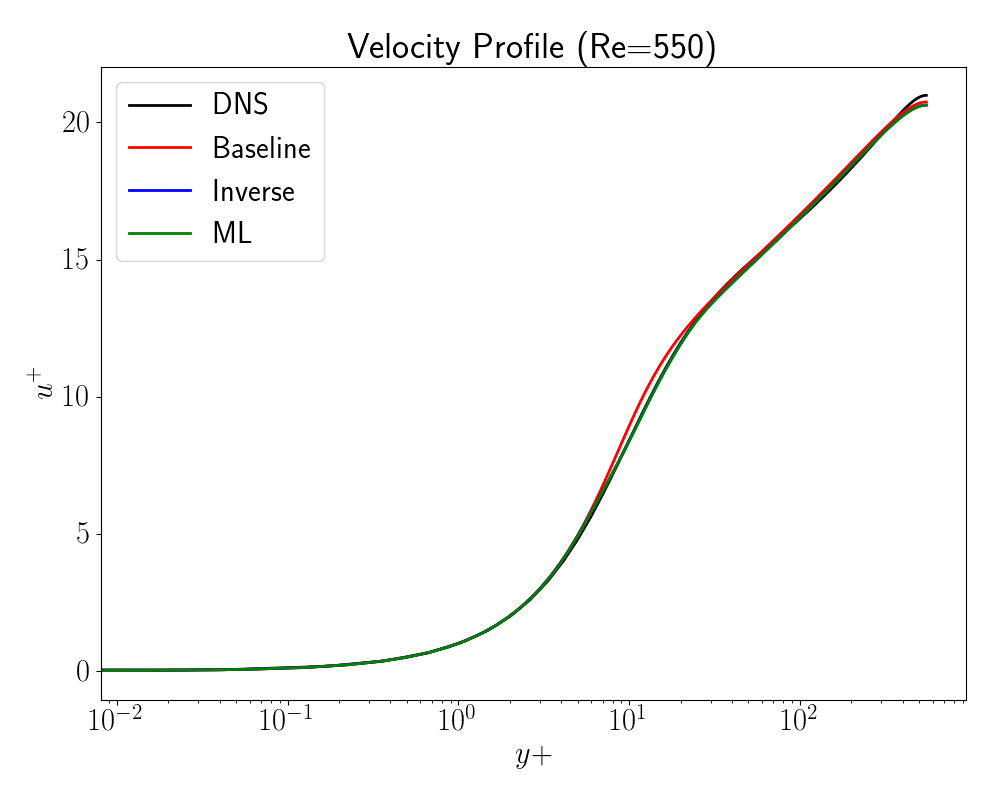
\includegraphics[width=0.32\textwidth]{images/Classic_Channel_SA_VelObj_RFtr/figs_SA_3_550/1.png}          %
}                                                                                                                 %
\subfloat[][Velocity Gradient profile]                                                                                          %
{                                                                                                                 %
    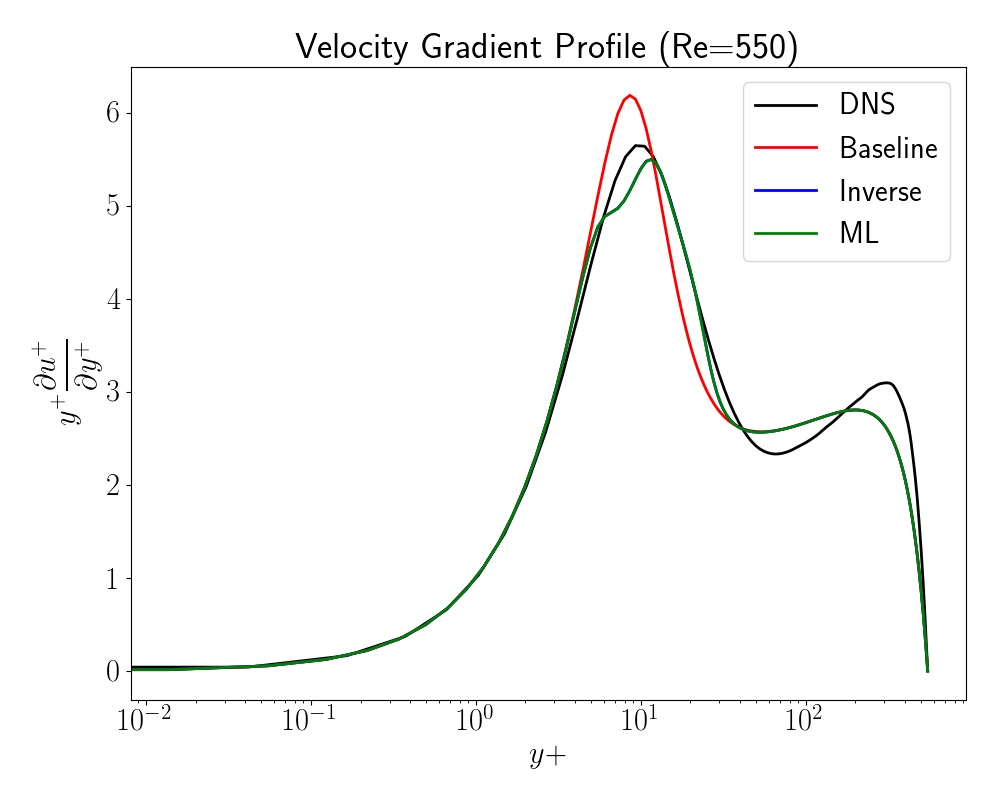
\includegraphics[width=0.32\textwidth]{images/Classic_Channel_SA_VelObj_RFtr/figs_SA_3_550/2.png}          %
}                                                                                                                 %

\subfloat[][Velocity profile]                                                                                          %
{                                                                                                                 %
    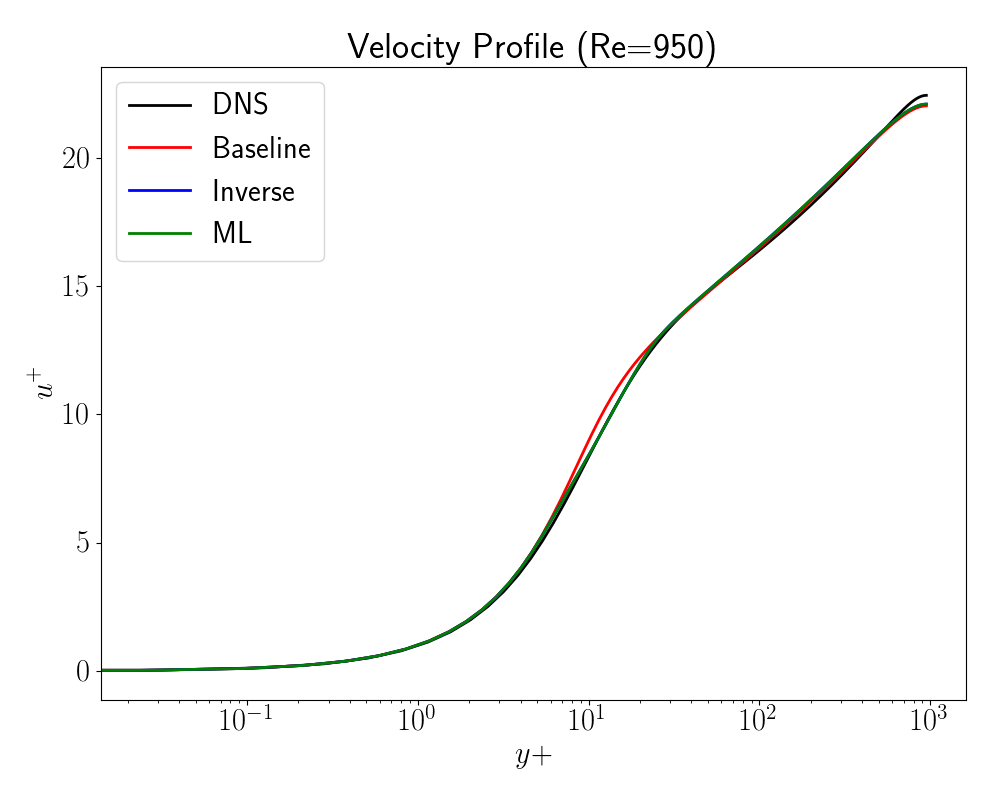
\includegraphics[width=0.32\textwidth]{images/Classic_Channel_SA_VelObj_RFtr/figs_SA_3_950/1.png}          %
}                                                                                                                 %
\subfloat[][Velocity Gradient profile]                                                                                          %
{                                                                                                                 %
    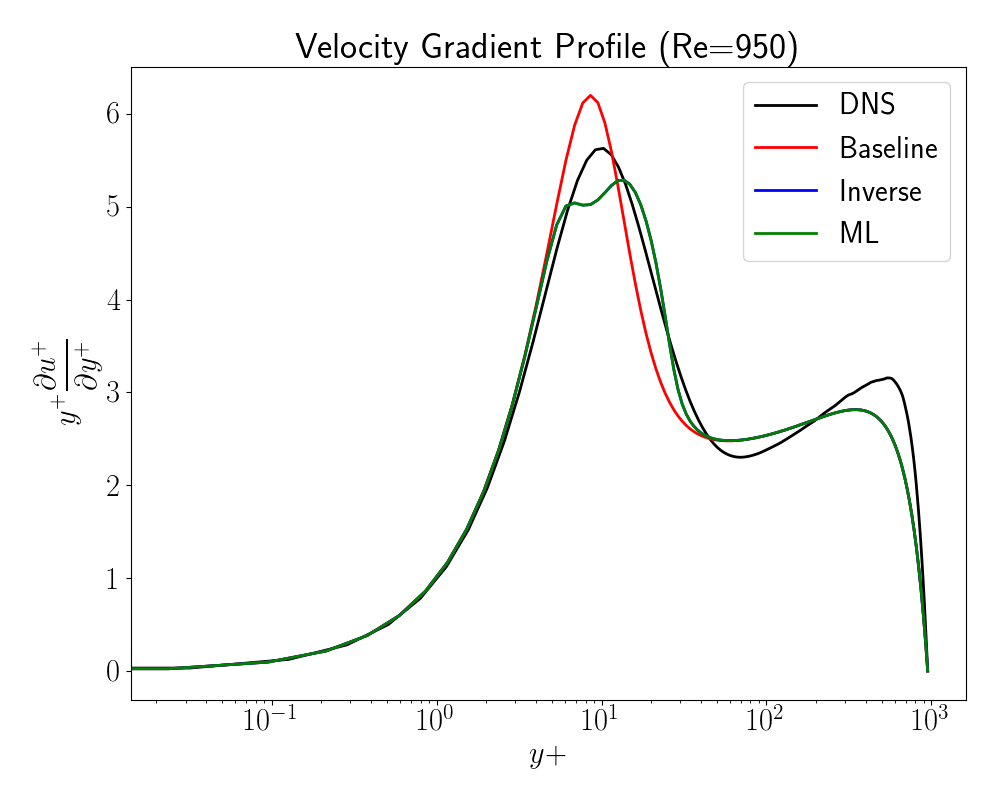
\includegraphics[width=0.32\textwidth]{images/Classic_Channel_SA_VelObj_RFtr/figs_SA_3_950/2.png}          %
}                                                                                                                 %
                                                                                                                  %
\caption{Velocity and Velocity Gradient Profiles}                                                                                       %
\label{vel1}                                                                                                     %
\end{figure}                                                                                                      %
                                                                                                                  %
%==================================================================================================================
%==================================================================================================================
                                                                                                                  %
\begin{figure}[H]                                                                                                 %
\centering                                                                                                        %
\subfloat[][Velocity profile]                                                                                          %
{                                                                                                                 %
    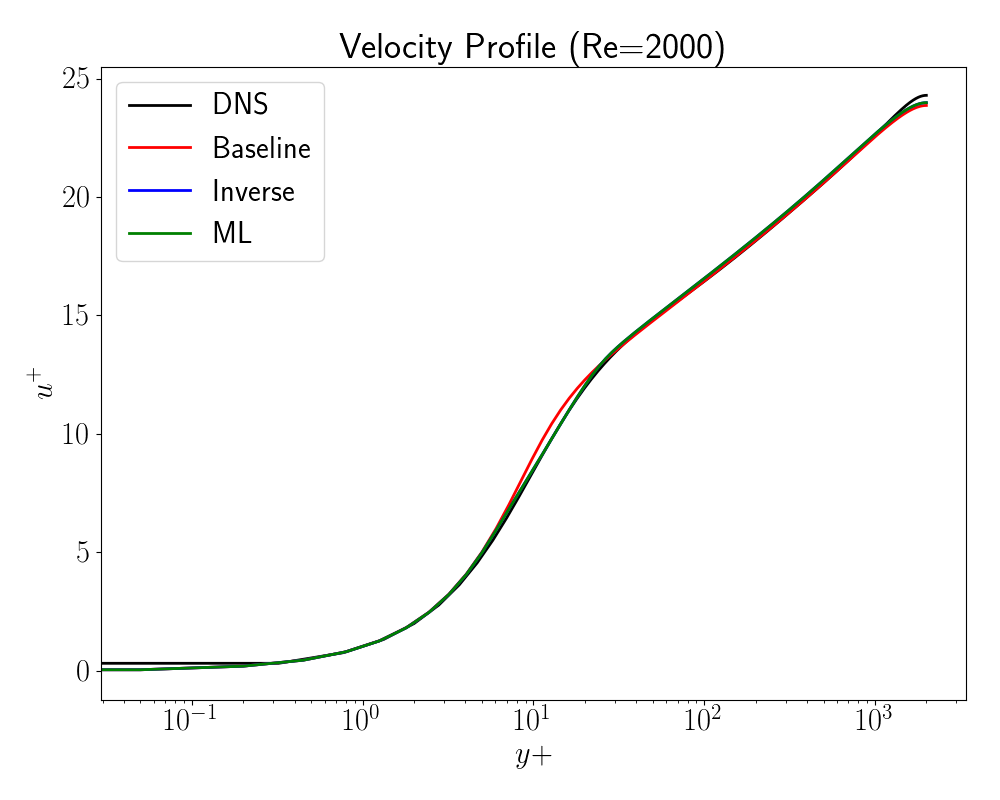
\includegraphics[width=0.32\textwidth]{images/Classic_Channel_SA_VelObj_RFtr/figs_SA_3_2000/1.png}          %
}                                                                                                                 %
\subfloat[][Velocity Gradient profile]                                                                                          %
{                                                                                                                 %
    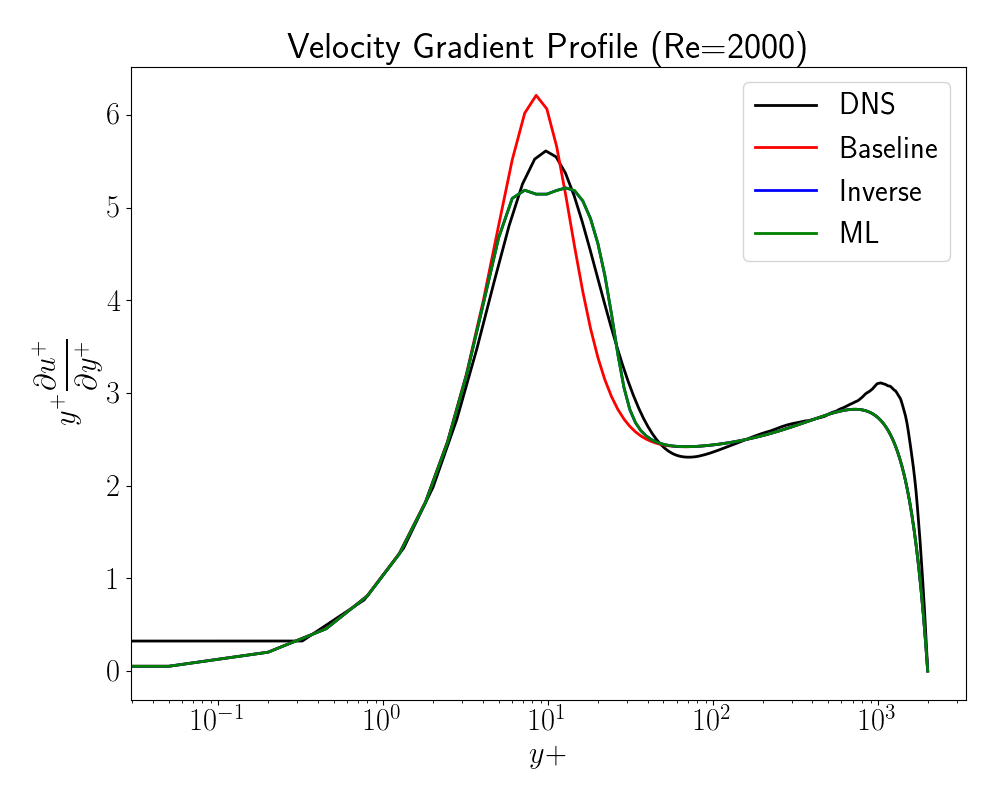
\includegraphics[width=0.32\textwidth]{images/Classic_Channel_SA_VelObj_RFtr/figs_SA_3_2000/2.png}          %
}                                                                                                                 %

\subfloat[][Velocity profile]                                                                                          %
{                                                                                                                 %
    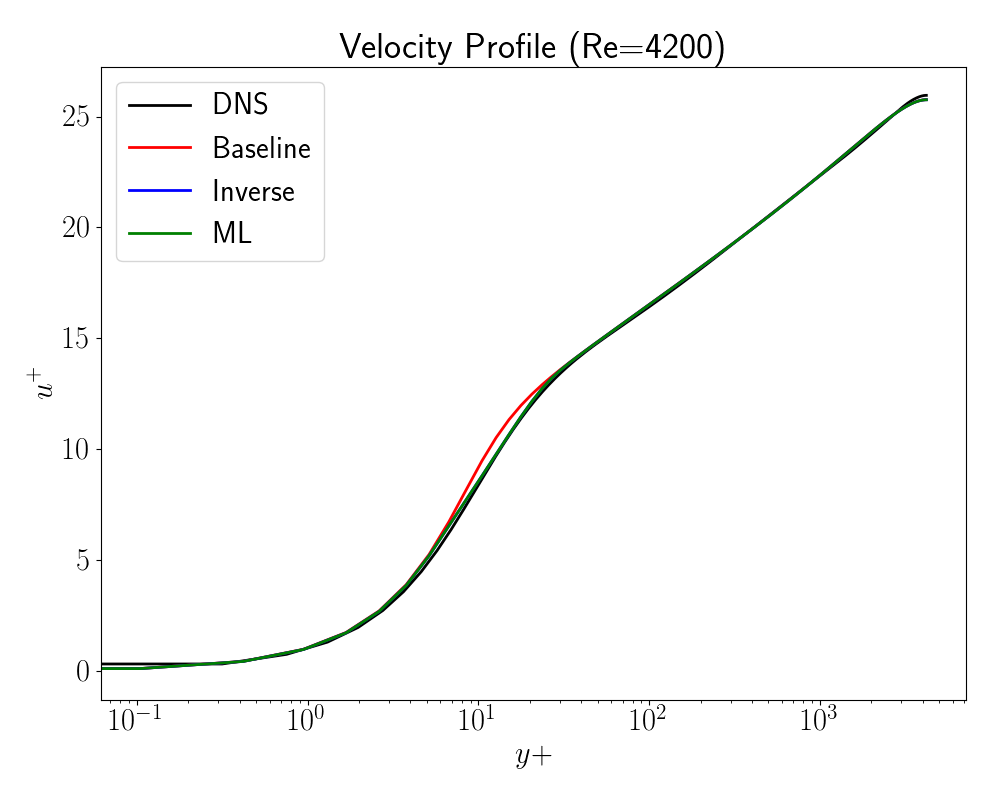
\includegraphics[width=0.32\textwidth]{images/Classic_Channel_SA_VelObj_RFtr/figs_SA_3_4200/1.png}          %
}                                                                                                                 %
\subfloat[][Velocity Gradient profile]                                                                                          %
{                                                                                                                 %
    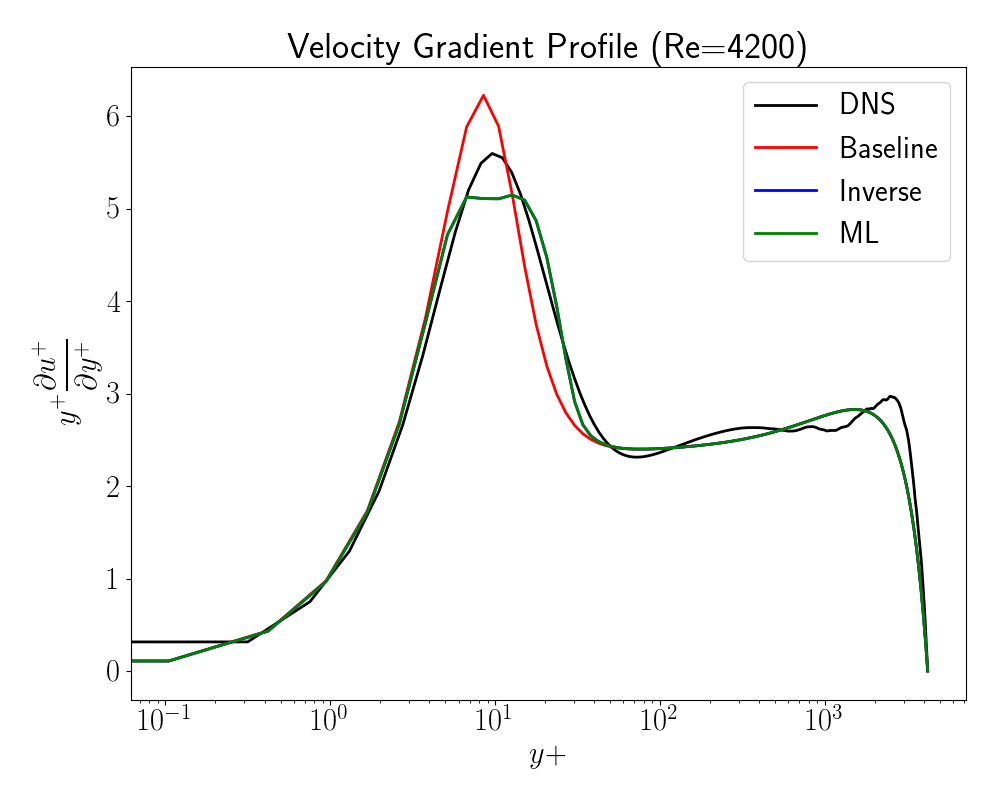
\includegraphics[width=0.32\textwidth]{images/Classic_Channel_SA_VelObj_RFtr/figs_SA_3_4200/2.png}          %
}                                                                                                                 %

\subfloat[][Velocity profile]                                                                                          %
{                                                                                                                 %
    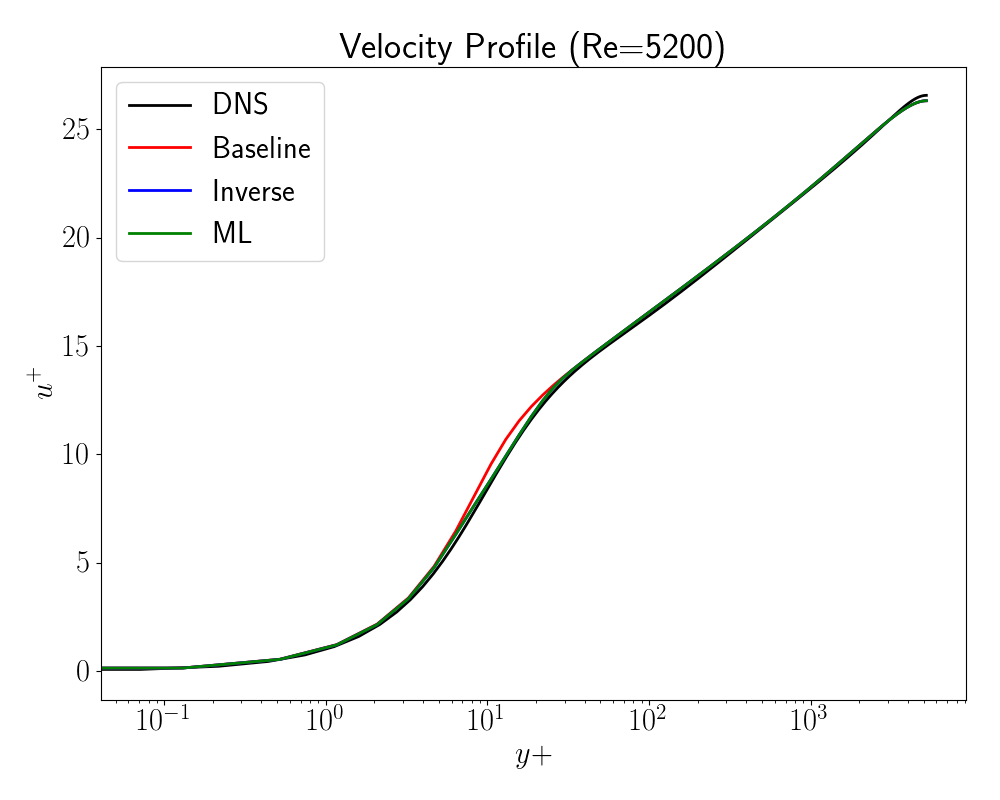
\includegraphics[width=0.32\textwidth]{images/Classic_Channel_SA_VelObj_RFtr/figs_SA_3_5200/1.png}          %
}                                                                                                                 %
\subfloat[][Velocity Gradient profile]                                                                                          %
{                                                                                                                 %
    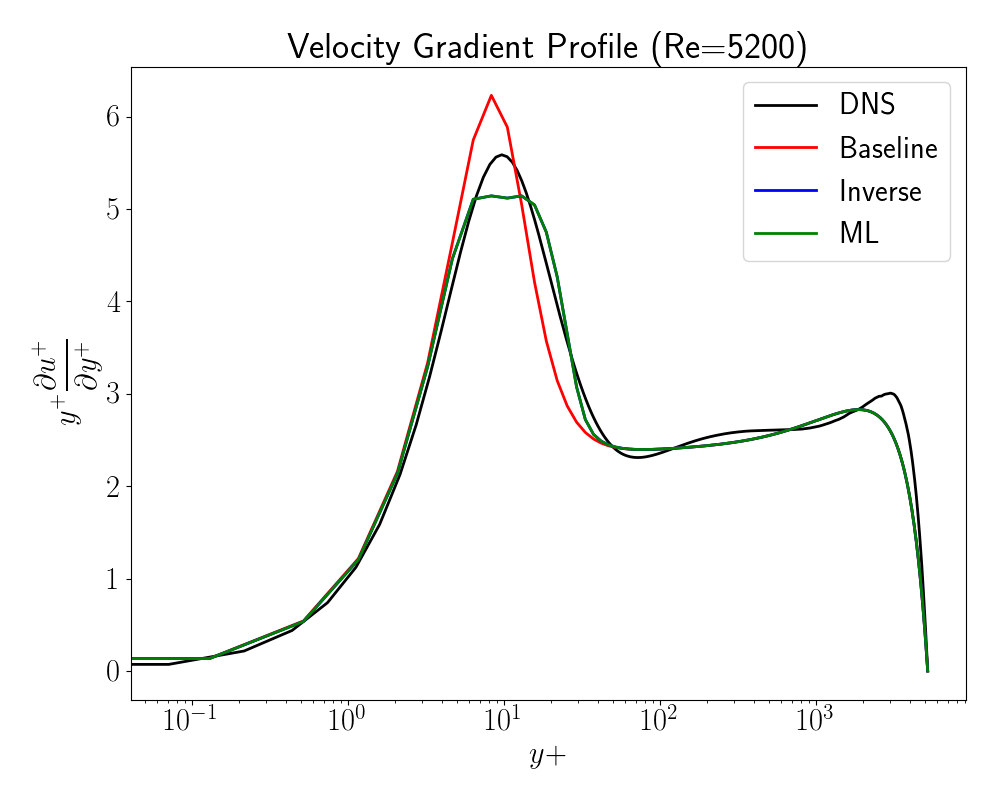
\includegraphics[width=0.32\textwidth]{images/Classic_Channel_SA_VelObj_RFtr/figs_SA_3_5200/2.png}          %
}                                                                                                                 %

\caption{Velocity and Velocity Gradient Profiles}                                                                                       %
\label{vel2}                                                                                                     %
\end{figure}                                                                                                      %
                                                                                                                  %
%==================================================================================================================
Note here that the beta profiles are almost identical in the $y^+$ (wall) coordinates, which means that the correction
is nearly constant across Reynolds numbers.

\subsection*{FIML-Classic augmentation of the 1st kind}
%==================================================================================================================
                                                                                                                  %
\begin{figure}[H]                                                                                                 %
\centering                                                                                                        %
\subfloat[][Optimization Convergence]                                                                                         %
{                                                                                                                 %
    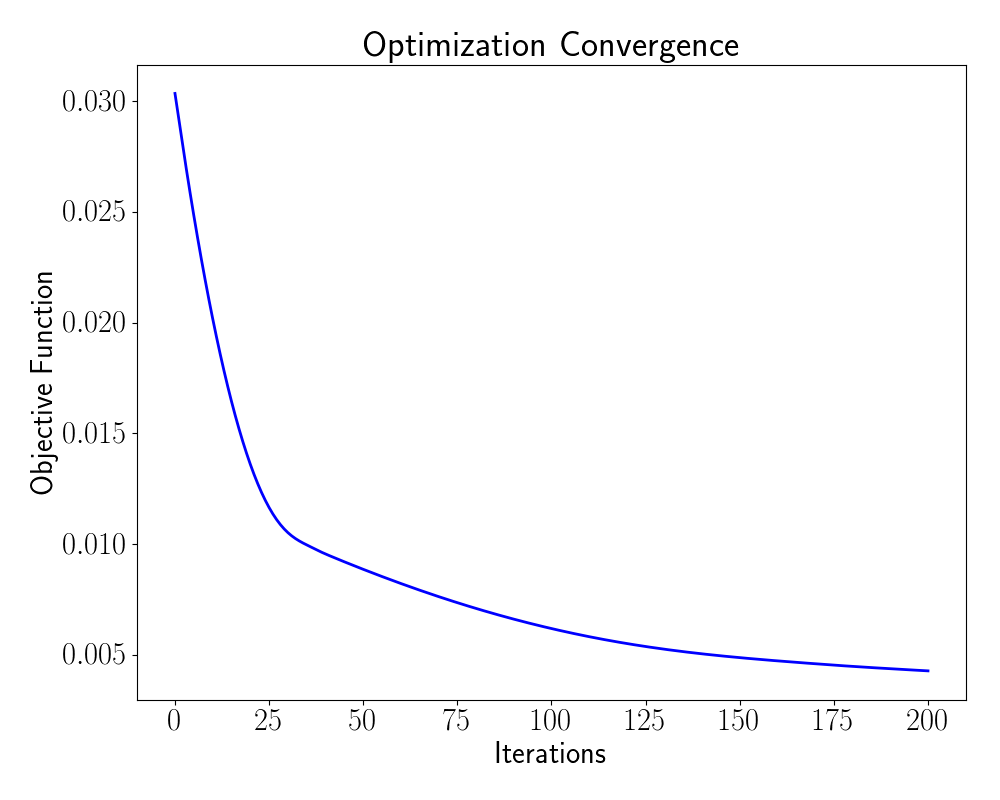
\includegraphics[width=0.32\textwidth]{images/figs/1_SA_1.png}         %
}                                                                                                                 %
%\subfloat[][ML Convergence]                                                                                        %
%{                                                                                                                 %
%    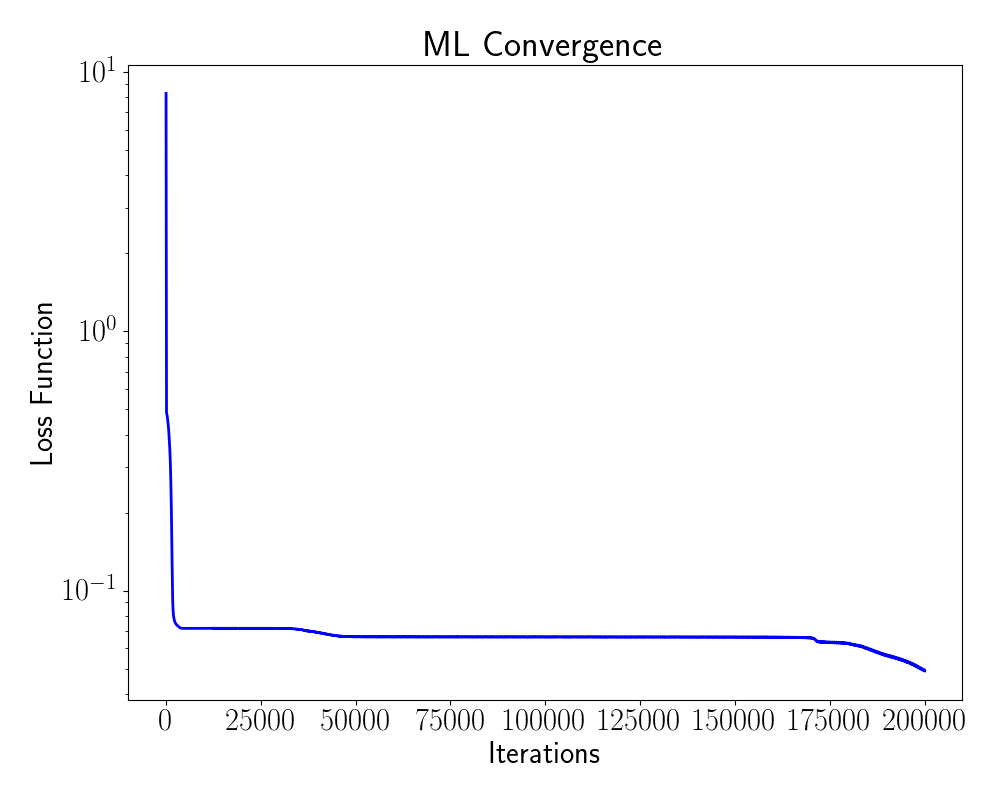
\includegraphics[width=0.32\textwidth]{images/figs/11_SA_1.png}        %
%}                                                                                                                 %
\subfloat[][Augmentation variable profile]                                                                                          %
{                                                                                                                 %
    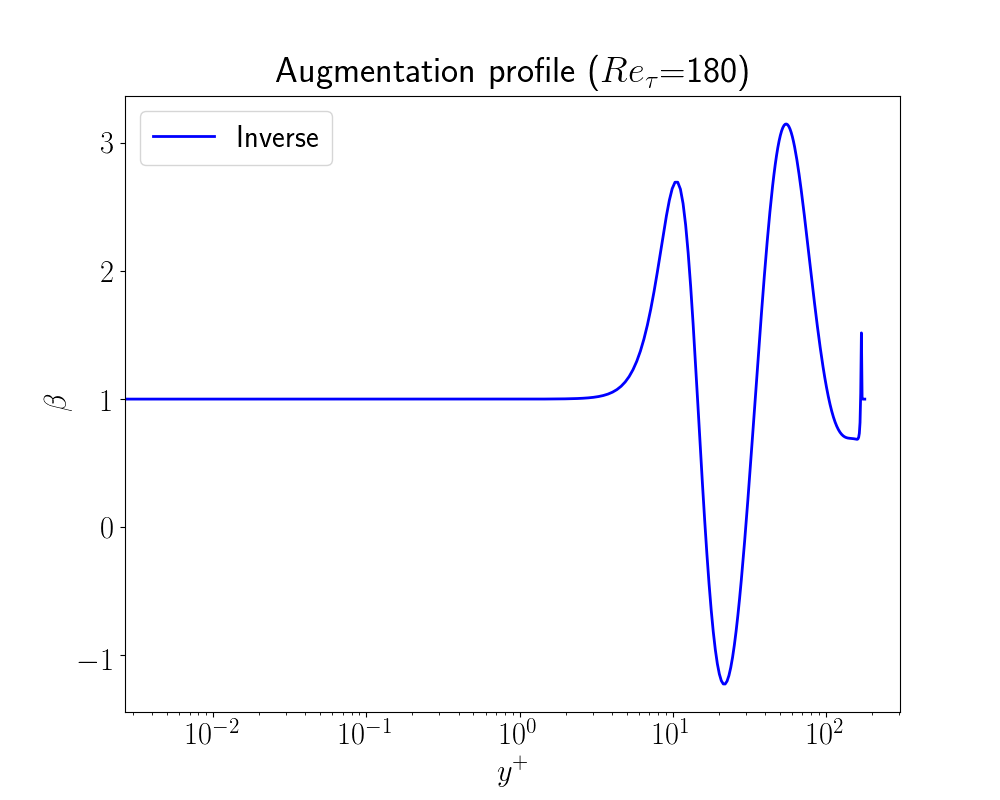
\includegraphics[width=0.32\textwidth]{images/figs_180_1/1000.png}          %
}                                                                                                                 %

\subfloat[][Optimization Convergence]                                                                                         %
{                                                                                                                 %
    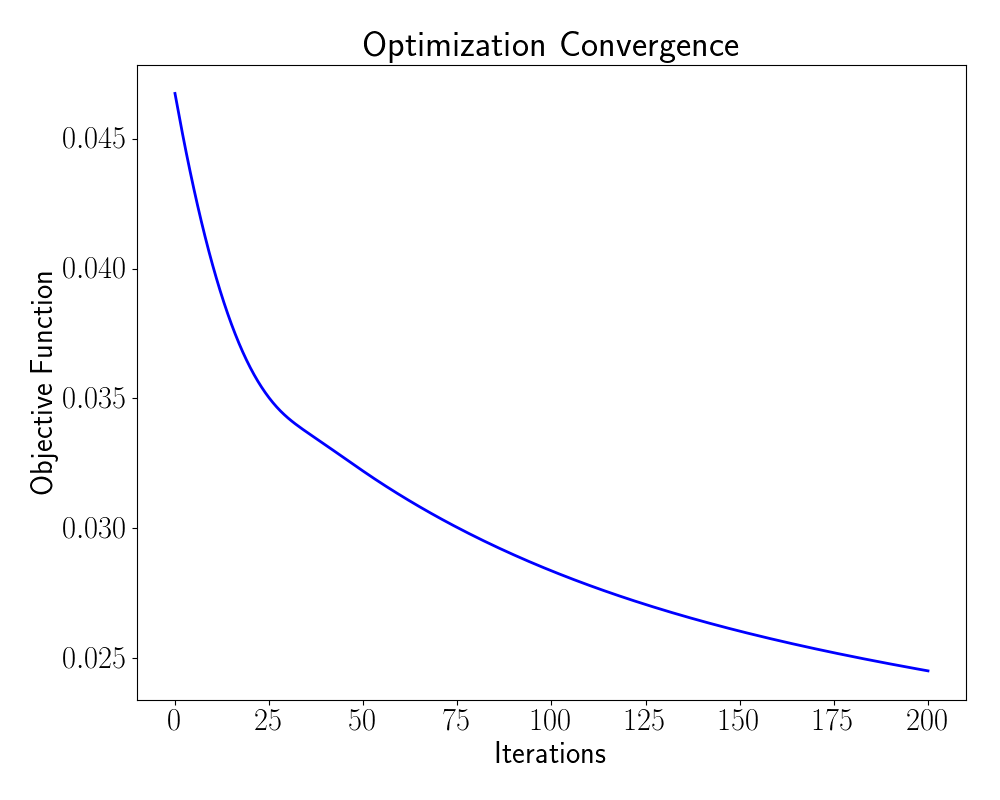
\includegraphics[width=0.32\textwidth]{images/figs/2_SA_1.png}         %
}                                                                                                                 %
%\subfloat[][ML Convergence]                                                                                        %
%{                                                                                                                 %
%    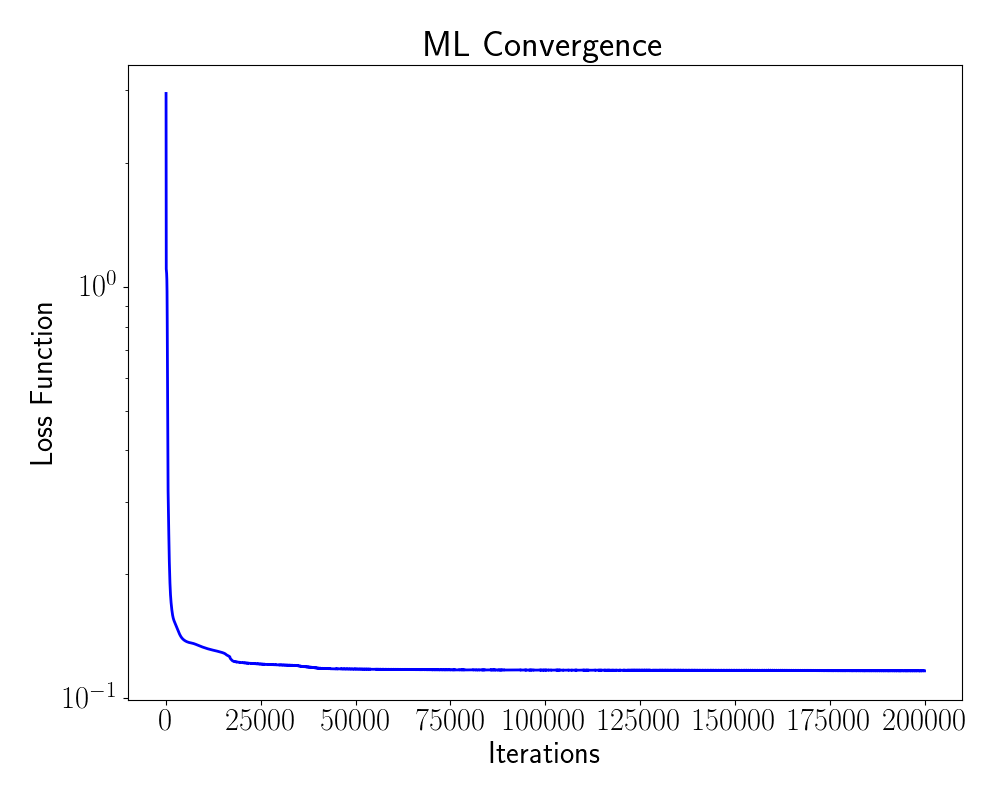
\includegraphics[width=0.32\textwidth]{images/figs/21_SA_1.png}        %
%}                                                                                                                 %
\subfloat[][Augmentation variable profile]                                                                                          %
{                                                                                                                 %
    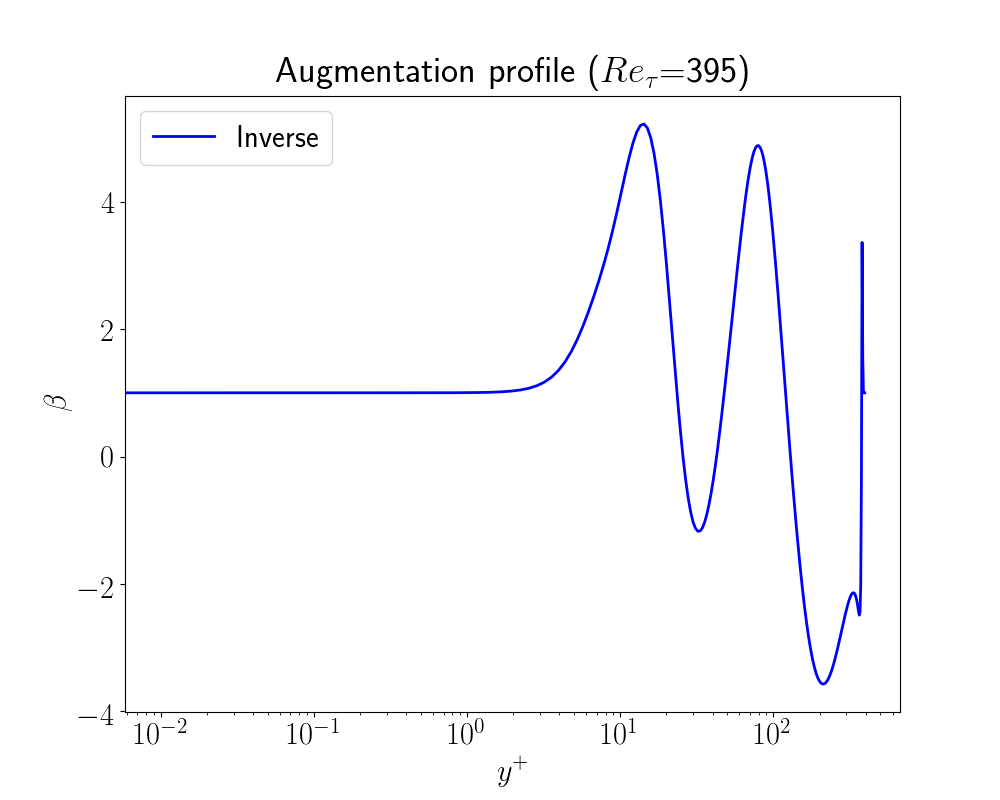
\includegraphics[width=0.32\textwidth]{images/figs_395_1/1000.png}          %
}                                                                                                                 %

\subfloat[][Optimization Convergence]                                                                                         %
{                                                                                                                 %
    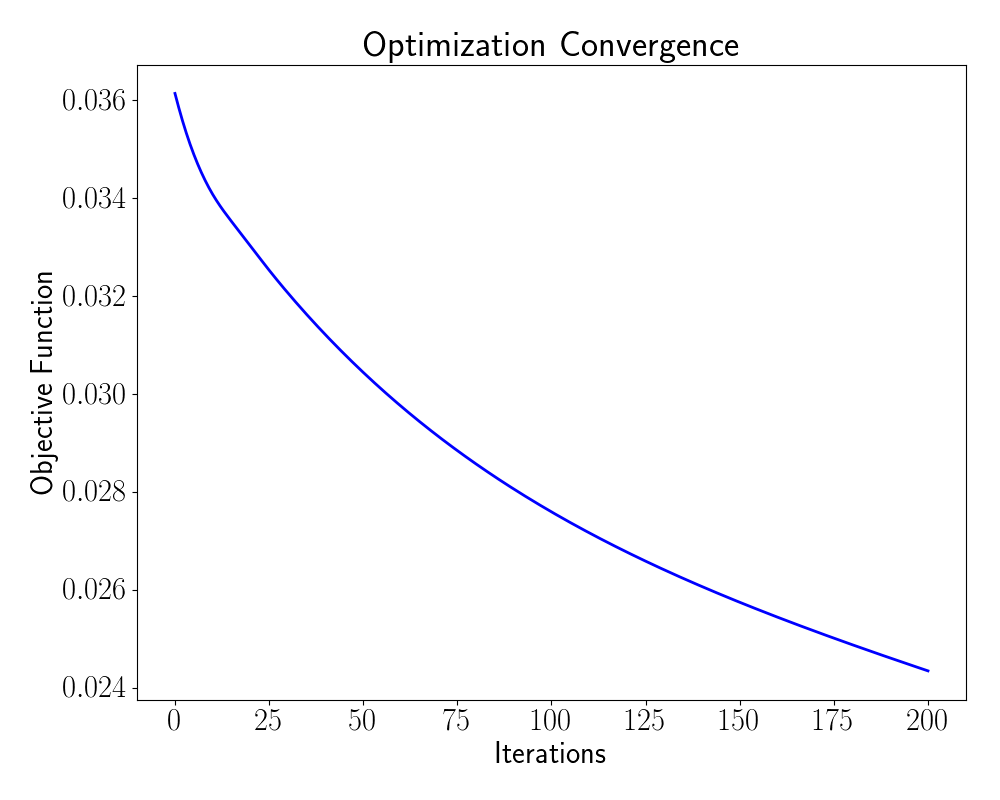
\includegraphics[width=0.32\textwidth]{images/figs/3_SA_1.png}         %
}                                                                                                                 %
%\subfloat[][ML Convergence]                                                                                        %
%{                                                                                                                 %
%    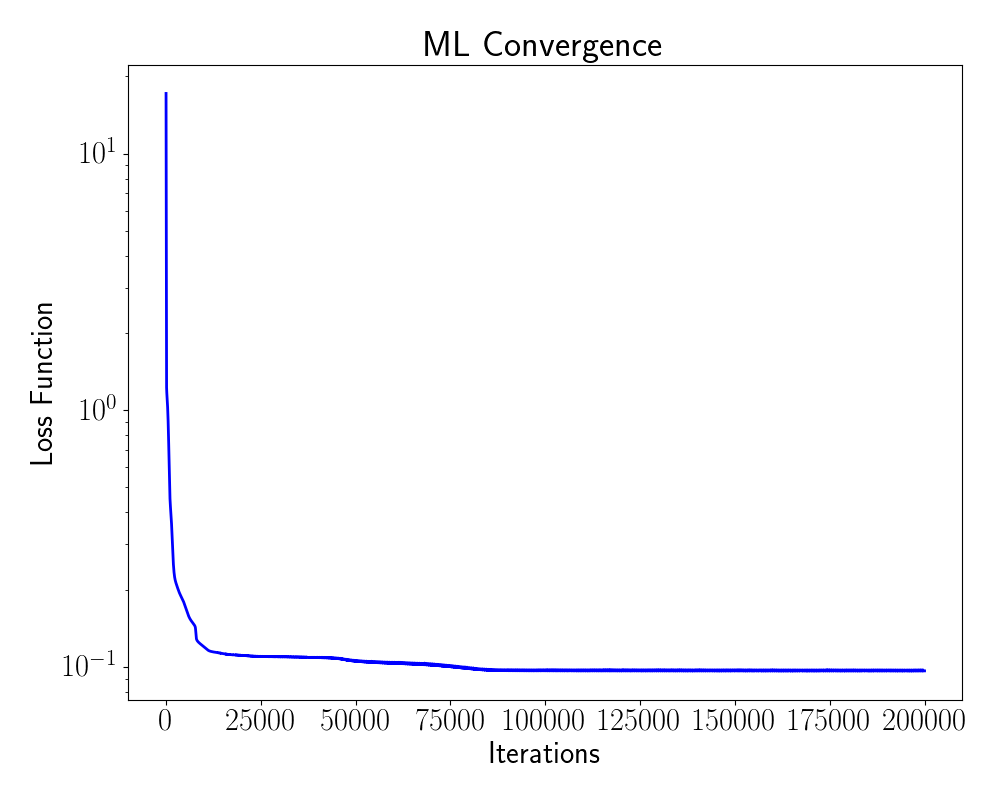
\includegraphics[width=0.32\textwidth]{images/figs/31_SA_1.png}        %
%}                                                                                                                 %
\subfloat[][Augmentation variable profile]                                                                                          %
{                                                                                                                 %
    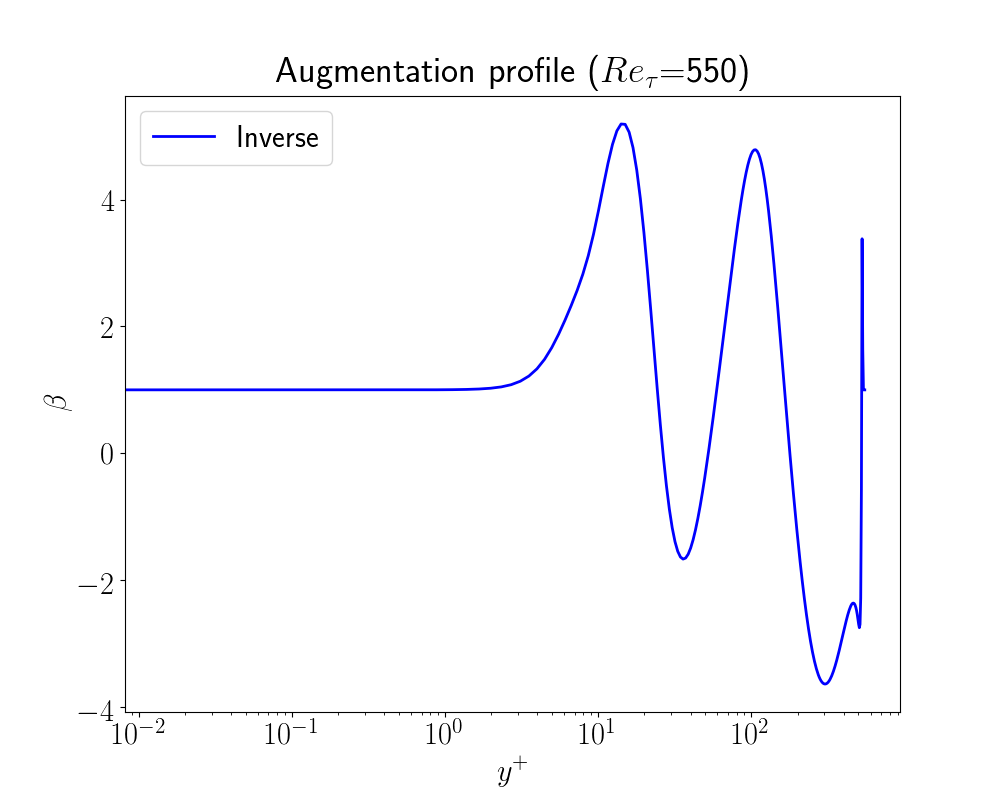
\includegraphics[width=0.32\textwidth]{images/figs_550_1/1000.png}          %
}                                                                                                                 %

\caption{Convergence and beta plots}                                                                                       %
\label{convbeta1}                                                                                                     %
\end{figure}                                                                                                      %
                                                                                                                  %
%==================================================================================================================
\pagebreak
%==================================================================================================================
                                                                                                                  %
\begin{figure}[H]                                                                                                 %
\centering                                                                                                        %
\subfloat[][Velocity profile]                                                                                          %
{                                                                                                                 %
    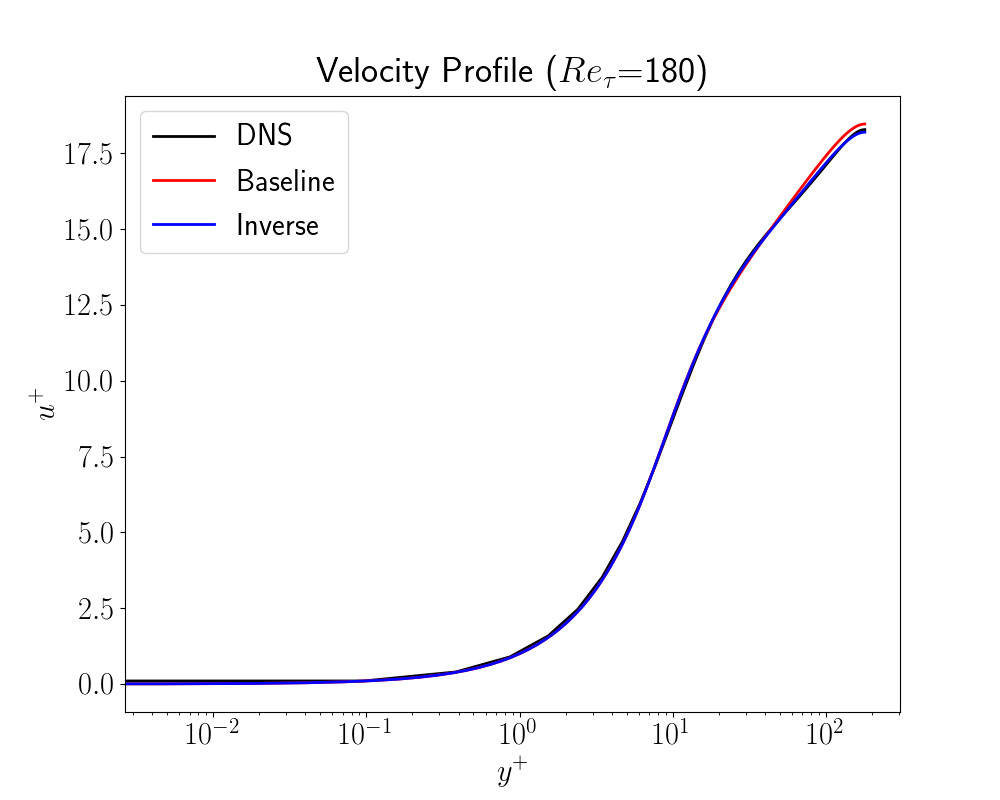
\includegraphics[width=0.32\textwidth]{images/figs_180_1/1.png}          %
}                                                                                                            %
\subfloat[][Velocity Gradient profile]                                                                                     %
{                                                                                                            %
    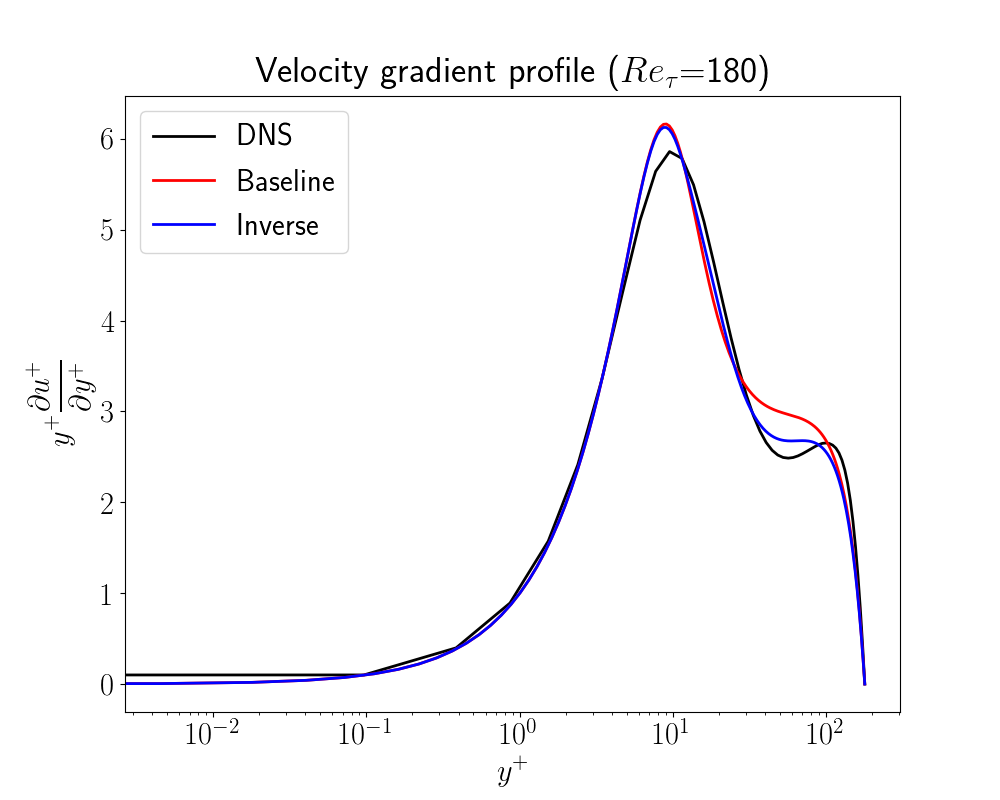
\includegraphics[width=0.32\textwidth]{images/figs_180_1/10.png}          %
}                                                                                                            %

\subfloat[][Velocity profile]                                                                                     %
{                                                                                                            %
    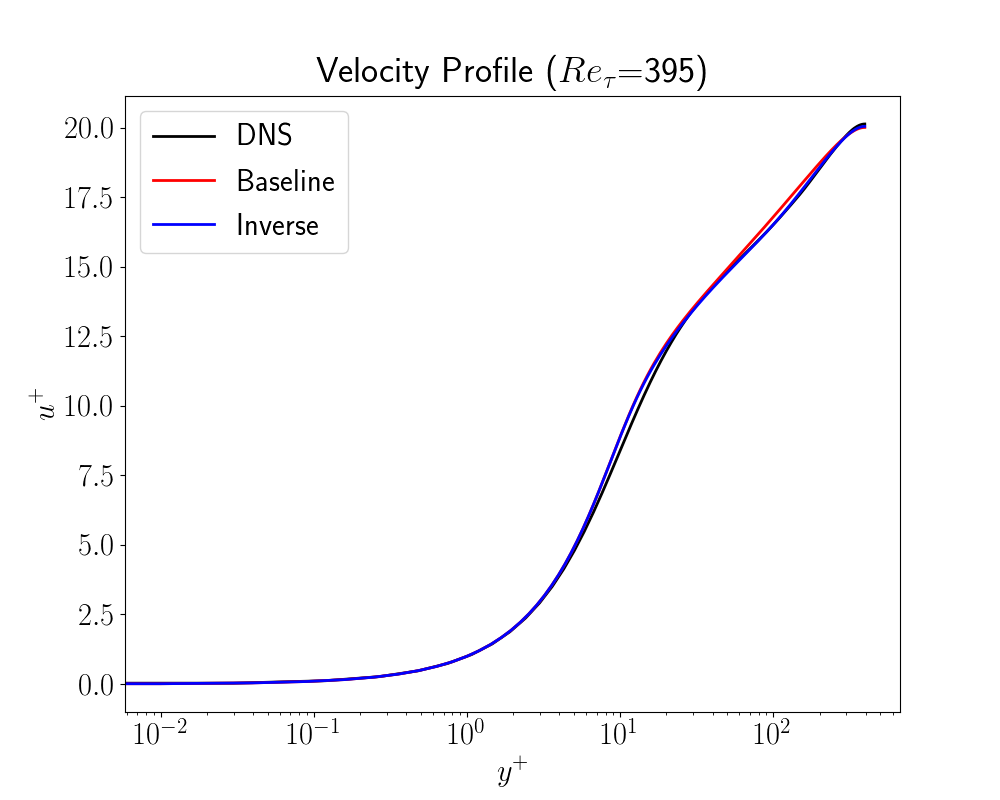
\includegraphics[width=0.32\textwidth]{images/figs_395_1/1.png}          %
}                                                                                                            %
\subfloat[][Velocity Gradient profile]                                                                                     %
{                                                                                                            %
    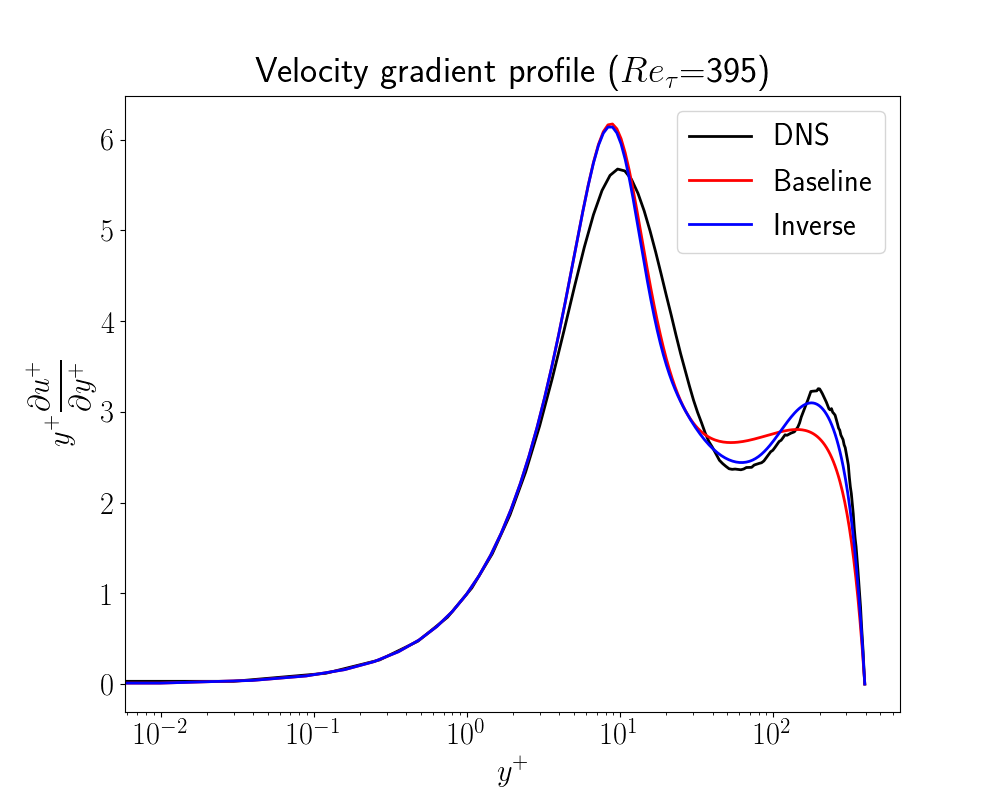
\includegraphics[width=0.32\textwidth]{images/figs_395_1/10.png}          %
}                                                                                                            %

\subfloat[][Velocity profile]                                                                                     %
{                                                                                                            %
    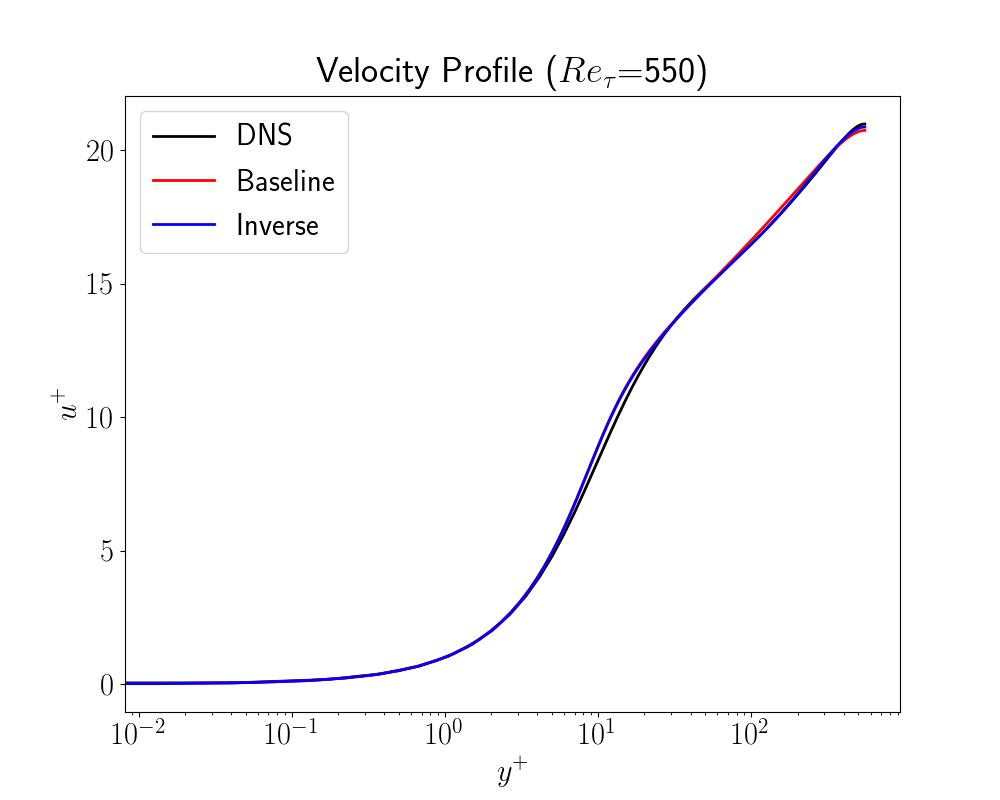
\includegraphics[width=0.32\textwidth]{images/figs_550_1/1.png}          %
}                                                                                                            %
\subfloat[][Velocity Gradient profile]                                                                                     %
{                                                                                                            %
    \includegraphics[width=0.32\textwidth]{images/figs_550_1/10.png}          %
}                                                                                                                 %

\caption{Velocity and Velocity Gradient Profiles}                                                                                       %
\label{vel2}                                                                                                     %
\end{figure}                                                                                                      %
                                                                                                                  %
%==================================================================================================================
As can be seen in the above plots, since the major discrepancy here is in the buffer layer, this augmentation struggles
to correct the profile as well as the previous one and shows large and even negative values for the augmentation factor.
Hence, it will be much efficient to correct the terms individually for the zones that need to be corrected.

\subsection*{FIML-Classic augmentation of the 4th kind}
%==================================================================================================================
                                                                                                                  %
\begin{figure}[H]                                                                                                 %
\centering                                                                                                        %
\subfloat[][Optimization Convergence]                                                                                         %
{                                                                                                                 %
    \includegraphics[width=0.32\textwidth]{images/figs_180_4/0.png}         %
}                                                                                                                 %
%\subfloat[][ML Convergence]                                                                                        %
%{                                                                                                                 %
%    \includegraphics[width=0.32\textwidth]{images/figs/11_SA_1.png}        %
%}                                                                                                                 %
\subfloat[][Augmentation variable profile]                                                                                          %
{                                                                                                                 %
    \includegraphics[width=0.32\textwidth]{images/figs_180_4/1000.png}          %
}                                                                                                                 %

\subfloat[][Optimization Convergence]                                                                                         %
{                                                                                                                 %
    \includegraphics[width=0.32\textwidth]{images/figs_395_4/0.png}         %
}                                                                                                                 %
%\subfloat[][ML Convergence]                                                                                        %
%{                                                                                                                 %
%    \includegraphics[width=0.32\textwidth]{images/figs/21_SA_1.png}        %
%}                                                                                                                 %
\subfloat[][Augmentation variable profile]                                                                                          %
{                                                                                                                 %
    \includegraphics[width=0.32\textwidth]{images/figs_395_4/1000.png}          %
}                                                                                                                 %

\subfloat[][Optimization Convergence]                                                                                         %
{                                                                                                                 %
    \includegraphics[width=0.32\textwidth]{images/figs_550_4/0.png}         %
}                                                                                                                 %
%\subfloat[][ML Convergence]                                                                                        %
%{                                                                                                                 %
%    \includegraphics[width=0.32\textwidth]{images/figs/31_SA_1.png}        %
%}                                                                                                                 %
\subfloat[][Augmentation variable profile]                                                                                          %
{                                                                                                                 %
    \includegraphics[width=0.32\textwidth]{images/figs_550_4/1000.png}          %
}                                                                                                                 %

\caption{Convergence and beta plots}                                                                                       %
\label{convbeta1}                                                                                                     %
\end{figure}                                                                                                      %
                                                                                                                  %
%==================================================================================================================
\pagebreak
%==================================================================================================================
                                                                                                                  %
\begin{figure}[H]                                                                                                 %
\centering                                                                                                        %
\subfloat[][Velocity profile]                                                                                          %
{                                                                                                                 %
    \includegraphics[width=0.32\textwidth]{images/figs_180_4/1.png}          %
}                                                                                                                 %
\subfloat[][Velocity Gradient profile]                                                                                          %
{                                                                                                                 %
    \includegraphics[width=0.32\textwidth]{images/figs_180_4/10.png}          %
}                                                                                                                 %

\subfloat[][Velocity profile]                                                                                          %
{                                                                                                                 %
    \includegraphics[width=0.32\textwidth]{images/figs_395_4/1.png}          %
}                                                                                                                 %
\subfloat[][Velocity Gradient profile]                                                                                          %
{                                                                                                                 %
    \includegraphics[width=0.32\textwidth]{images/figs_395_4/10.png}          %
}                                                                                                                 %

\subfloat[][Velocity profile]                                                                                          %
{                                                                                                                 %
    \includegraphics[width=0.32\textwidth]{images/figs_550_4/1.png}          %
}                                                                                                                 %
\subfloat[][Velocity Gradient profile]                                                                                          %
{                                                                                                                 %
    \includegraphics[width=0.32\textwidth]{images/figs_550_4/10.png}          %
}                                                                                                                 %

\caption{Velocity and Velocity Gradient Profiles}                                                                                       %
\label{vel2}                                                                                                     %
\end{figure}                                                                                                      %
                                                                                                                  %
%==================================================================================================================
Here too, the optimization tries to correct the buffer layer but isn't successful and leads to $\beta$ values of
a large magnitude than expected. Also, this augmentation neither respects the original calibration nor the law of the wall.
%================================================================================================================================================================================

\end{document}
